	% =======================================================
	%                 第 16 章：一般均衡与经济效率
	% =======================================================
	\chapter{一般均衡与经济效率}
	
	\section{复习题}
	\begin{enumerate}[label=\textbf{\arabic*.}, leftmargin=*]
		\item \textbf{为什么反馈效应能使一般均衡分析与局部均衡分析存在很大的不同？}
		
		\textbf{答：}
		局部均衡分析核心在于孤立地研究单一市场的供求与价格决定，将其他市场的交互影响视作外生常数。一般均衡分析法则将所有相互关联的市场视为有机整体，显性化考察各市场之间价格与数量的交互传导。反馈效应是指某一市场的初始失衡引起相关市场价格变动后，这种变动反过来又对原市场产生二次冲击的机制。
		
		以电影票和录像带租赁两个替代品市场为例，若政府对电影票征税，局部均衡仅关注电影票自身价格上涨或需求回落。然而一般均衡分析表明，电影票税收会引致消费者转向录像带市场并推高其价格，而录像带价格的上涨又会反向刺激电影票需求的回升。这种多市场价格的连锁调整与多轮贴合反馈，最终决定了所有市场的全局均衡，其结果往往大幅偏离局部均衡的预测。
		
		\begin{center}
			\small
			\renewcommand{\arraystretch}{1.0}
			\begin{tikzpicture}[x=0.60cm, y=0.60cm, >=stealth, thick, every node/.style={scale=0.85}]
				
				% ==================== 层层嵌套 1：左图（电影票市场） ====================
				% 1. 辅助虚线层（最底层）
				\draw[dashed, gray, thin] (0,2.0) -- (2.0,2.0) -- (2.0,0);
				\draw[dashed, gray, thin] (0,2.5) -- (2.5,2.5) -- (2.5,0);
				
				% 2. 坐标轴层
				\draw[->] (0,0) -- (4.5,0) node[below] {$Q_m$};
				\draw[->] (0,0) -- (0,4.5) node[left] {$P_m$};
				
				% 3. 供需实线层（精细裁切定义域，杜绝废线）
				\draw[domain=0.5:4.0] plot(\x, {4.0-\x}) node[above right=-2pt] {$D_m$};
				\draw[domain=0.8:4.2] plot(\x, {5.0-\x}) node[above right=-2pt] {$D'_m$};
				\draw[domain=0.5:3.8] plot(\x, {\x}) node[right] {$S_m$};
				
				% 4. 均衡交点与防重叠标签（最顶层）
				\fill (2.0,2.0) circle (1.8pt);
				\fill (2.5,2.5) circle (1.8pt);
				\node[left, fill=white, inner sep=1pt] at (0,2.0) {$P_1$};
				\node[left, fill=white, inner sep=1pt] at (0,2.5) {$P_2$};
				\node[below, fill=white, inner sep=1pt] at (2.0,0) {$Q_1$};
				\node[below, fill=white, inner sep=1pt] at (2.5,0) {$Q_2$};
				
				\node[below] at (2.0, -0.8) {(a) 电影票市场};
				
				% ==================== 层层嵌套 2：右图（录像带市场） ====================
				% 精确计算物理平移量（3.4cm），确保大图无缝紧凑并置，绝不溢出边界
				\begin{scope}[xshift=3.4cm]
					% 1. 辅助虚线层
					\draw[dashed, gray, thin] (0,1.8) -- (1.8,1.8) -- (1.8,0);
					\draw[dashed, gray, thin] (0,2.2) -- (2.2,2.2) -- (2.2,0);
					
					% 2. 坐标轴层
					\draw[->] (0,0) -- (4.5,0) node[below] {$Q_v$};
					\draw[->] (0,0) -- (0,4.5) node[left] {$P_v$};
					
					% 3. 供需实线层
					\draw[domain=0.5:3.6] plot(\x, {3.6-\x}) node[left,yshift=6pt,xshift=-6pt] {$D_v$};
					\draw[domain=0.5:4.0] plot(\x, {4.4-\x}) node[right] {$D'_v$};
					\draw[domain=0.5:3.8] plot(\x, {\x}) node[right] {$S_v$};
					
					% 4. 均衡交点与防重叠标签
					\fill (1.8,1.8) circle (1.8pt);
					\fill (2.2,2.2) circle (1.8pt);
					\node[left, fill=white, inner sep=1pt] at (0,1.6) {$Q_1$};
					\node[left, fill=white, inner sep=1pt] at (0,2.4) {$Q_2$};
					\node[below, fill=white, inner sep=1pt] at (1.8,0) {$X_1$};
					\node[below, fill=white, inner sep=1pt] at (2.2,0) {$X_2$};
					
					\node[below] at (2.0, -0.8) {(b) 录像带市场};
				\end{scope}
				
			\end{tikzpicture}
		\end{center}
		
		\item \textbf{解释埃奇沃思盒形图中的一点是如何同时代表两个消费者所拥有的商品配置的。}
		
		\textbf{答：}
		埃奇沃思盒形图通过双原点对顶的外框结构，将整个经济体中既定的两种商品总量进行了完美的几何约束。设第一种商品的总量为 $X'$，第二种商品的总量为 $Y'$，盒子的水平总长度与垂直总高度分别对应这两个总量。
		
		以左下角为消费者 A 的原点 $O_A$，从左向右和从下向上分别度量其对商品 X 和 Y 的消费量；以右上角为消费者 B 的原点 $O_B$，从右向左和从上向下分别度量其对商品 X 和 Y 的消费量。盒内任意一点 D 到四条边界的垂直距离，自动在两个对顶坐标系中映射出满足总资源约束的分配组合，从而唯一地代表两个消费者的商品配置。
		\[
		\begin{cases}
			X_a + X_b = X' \\
			Y_a + Y_b = Y'
		\end{cases}
		\]
		
		\begin{center}
			\small
			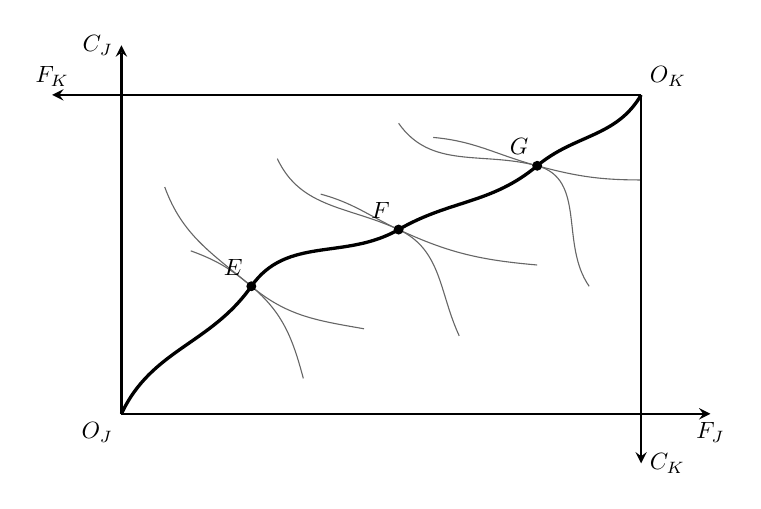
\begin{tikzpicture}[x=1.1cm, y=0.9cm, >=stealth, thick, every node/.style={scale=0.85}]
				% 1. 核心契约曲线绘制 (连接两原点，平滑曲折延伸)
				\draw[very thick] (0,0) to[out=65, in=235] (1.5,1.8) 
				to[out=55, in=210] (3.2,2.6) 
				to[out=30, in=220] (4.8,3.5) 
				to[out=40, in=240] (6,4.5);
				
				% 2. 消费者无差异曲线群 (采用切线斜率共轭锚定技术，确保完美相切)
				% 切点 E 处的切曲线对 (控制点切角一致设定为 in=140, out=-40)
				\draw[black!60, thin] (0.5,3.2) to[out=-70, in=140] (1.5,1.8) to[out=-40, in=170] (2.8,1.2);
				\draw[black!60, thin] (0.8,2.3) to[out=-20, in=140] (1.5,1.8) to[out=-40, in=105] (2.1,0.5);
				
				% 切点 F 处的切曲线对 (控制点切角一致设定为 in=155, out=-25)
				\draw[black!60, thin] (1.8,3.6) to[out=-65, in=155] (3.2,2.6) to[out=-25, in=175] (4.8,2.1);
				\draw[black!60, thin] (2.3,3.1) to[out=-15, in=155] (3.2,2.6) to[out=-25, in=115] (3.9,1.1);
				
				% 切点 G 处的切曲线对 (控制点切角一致设定为 in=165, out=-15)
				\draw[black!60, thin] (3.2,4.1) to[out=-55, in=165] (4.8,3.5) to[out=-15, in=180] (6.0,3.3);
				\draw[black!60, thin] (3.6,3.9) to[out=-5, in=165] (4.8,3.5) to[out=-15, in=125] (5.4,1.8);
				
				% 3. 双向学术标准坐标轴 (封闭盒式矩阵架构)
				% 詹姆斯 (James) 坐标轴
				\draw[->] (0,0) -- (6.8,0) node[below] {$F_J$};
				\draw[->] (0,0) -- (0,5.2) node[left] {$C_J$};
				
				% 凯伦 (Karen) 坐标轴
				\draw[->] (6,4.5) -- (-0.8,4.5) node[above] {$F_K$};
				\draw[->] (6,4.5) -- (6,-0.7) node[right] {$C_K$};
				
				% 4. 关键均衡点与原点几何标号 (利用 fill=white 净化背景噪音)
				\node[below left] at (0,0) {$O_J$};
				\node[above right] at (6,4.5) {$O_K$};
				
				\fill (1.5,1.8) circle (1.8pt);
				\node[above left, yshift=1pt] at (1.5,1.8) {$E$};
				
				\fill (3.2,2.6) circle (1.8pt);
				\node[above left, yshift=1pt] at (3.2,2.6) {$F$};
				
				\fill (4.8,3.5) circle (1.8pt);
				\node[above left, yshift=1pt] at (4.8,3.5) {$G$};
			\end{tikzpicture}
		\end{center}
		
		\item \textbf{在埃奇沃思盒形图的交换分析中，解释为什么在契约曲线上的每一点，两个消费者的边际替代率都相等。}
		
		\textbf{答：}
		交换契约曲线在几何上被定义为两个消费者的一系列无差异曲线切点的连续轨迹。根据微观经济学定义，在特定的无差异曲线上，任意一点的切线斜率的绝对值即为消费者对这两种商品的边际替代率。
		
		当两个消费者的无差异曲线在盒形图内部某点达成几何相切时，它们在该点共同分享唯一的一条公切线，这意味着两者的无差异曲线斜率在切点处必然严格相等。在偏好满足严格凸性的假设下，无差异曲线的相切状态即代数对应着边际替代率的完全一致，因此契约曲线上的每一点都满足该效率特征。
		\[
		MRS_A = MRS_B
		\]
		
		\item \textbf{“因为契约曲线上的所有点都是有效率的，因此从社会的观点来看它们都是同样合意的。”你同意这种说法吗？请加以解释。}
		
		\textbf{答：}
		不同意这种说法。交换契约曲线上的点全部具备帕累托最优效率，这意味着在不使任何他人福利受损的前提下，社会已经无法再增加任何人的福利，但这一纯粹的效率评判标准完全忽略了公平原则。
		
		事实上，契约曲线上包含着无穷多个有效的分配组合，其中甚至包含财富分配极度不平等的极端状态。例如在契约曲线的两个对角端点上，所有的社会资源均被单一个体垄断，另一体福利为零，这从社会规范福利的角度来看显然是极不合意的。
		
		\item \textbf{效用可能性边界是如何与契约曲线相联系的？}
		
		\textbf{答：}
		效用可能性边界是交换契约曲线从商品配置空间向效用空间进行拓扑映射的直接产物。契约曲线上的每一个最优配置点，都包含着两个消费者相互对应的序数效用水平组合。
		
		通过提取契约曲线上各切点的效用数值，并以两位消费者的效用水平作为横纵坐标轴，即可在效用空间中描绘出一条向下倾斜的边界线。该边界线上的每一个几何位点与契约曲线上的效率切点存在着一一对应关系，直观反映了在资源总量和偏好既定下，两位消费者福利此消彼长的边界约束。
		
		\begin{center}
			\small
			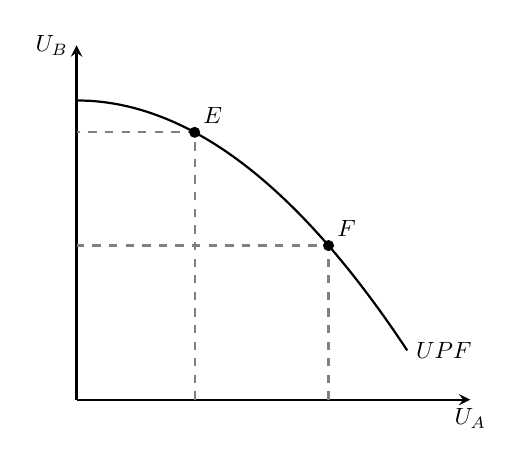
\begin{tikzpicture}[x=1.0cm, y=1.0cm, >=stealth, thick, every node/.style={scale=0.85}]
				% 坐标轴
				\draw[->] (0,0) -- (5.0,0) node[below] {$U_A$};
				\draw[->] (0,0) -- (0,4.5) node[left] {$U_B$};
				
				% 边界曲线
				\draw[smooth, domain=0:4.2] plot (\x, {3.8 - 0.18*\x*\x}) node[right] {$UPF$};
				
				% 典型契约点映射
				\coordinate (E) at (1.5, 3.395);
				\coordinate (F) at (3.2, 1.957);
				
				\draw[dashed, gray] (1.5,0) -- (1.5,3.395) -- (0,3.395);
				\draw[dashed, gray] (3.2,0) -- (3.2,1.957) -- (0,1.957);
				
				\fill (E) circle (2pt) node[above right] {$E$};
				\fill (F) circle (2pt) node[above right] {$F$};
			\end{tikzpicture}
		\end{center}
		
		\item \textbf{在埃奇沃思生产盒形图中，要使配置处在契约曲线上，必须具备什么条件？为什么竞争性均衡是在契约曲线上的？}
		
		\textbf{答：}
		在埃奇沃思生产盒形图中，要使要素配置处在生产契约曲线上，任何一对生产要素之间的边际技术替代率在所有商品的生产中都必须严格相等。这意味着用劳动与资本生产商品 X 时的边际技术替代率，必须等于生产商品 Y 时的边际技术替代率。此时全社会的要素配置达到了帕累托最优状态，实现了生产的一般均衡，连接所有此类高效率切点的轨迹即构成了生产契约曲线。
		\[
		MRTS_{LK}^{X} = MRTS_{LK}^{Y}
		\]
		
		在完全竞争的市场环境下，每种生产要素的价格对于所有的生产者而言都是完全相同的。追求利润最大化的厂商一定会主动调整要素投入组合，使得要素的边际技术替代率等于要素市场的相对价格之比。由于所有厂商在均衡时面对相同的要素价格比率，各商品生产中的边际技术替代率自发趋于相等，因此竞争性均衡必然位于生产契约曲线之上。
		
		\item \textbf{生产可能性边界是如何与生产契约曲线相联系的？}
		
		\textbf{答：}
		生产可能性边界描绘了在技术水平与要素总量既定的条件下，整个经济体所能生产的各种产品最大产量的组合轨迹。这一重要的效率边界是通过生产契约曲线直接拓扑映射而来的。
		
		生产契约曲线上的每一个切点不仅代表了劳动和资本在两个商品部门之间的帕累托最优配置，同时也唯一对应着该要素组合下两种商品的最优产出水平。将契约曲线上的要素投入组合转换为对应的实物产量，并投影到以产品产量为坐标轴的商品空间中，便得到了光滑的生产可能性边界。
		
		\item \textbf{什么是边际转换率？为什么一种商品对另一种商品的边际转换率等于生产两种商品的边际成本之比？}
		
		\textbf{答：}
		边际转换率衡量了在社会资源与生产技术既定的条件下，为了多生产某一单位的某种商品而必须放弃的另一种商品的数量。在几何上，边际转换率表现为生产可能性边界曲线上某一点切线斜率的绝对值。
		\[
		MRT_{XY} = \left| \frac{\mathrm{d}Y}{\mathrm{d}X} \right|
		\]
		
		在生产可能性边界上移动时，由于投入要素总量固定，增加商品 X 引起的总成本增加必须等于减少商品 Y 所释放的成本空间。这意味着增加商品 X 的边际成本与变动量之积，在数值上等于减少商品 Y 的边际成本与变动量之积。通过代数变形可知，两商品产量变动的比率绝对值必然等于它们的边际成本之比。
		\[
		MC_X \cdot \mathrm{d}X + MC_Y \cdot \mathrm{d}Y = 0 \implies \left| \frac{\mathrm{d}Y}{\mathrm{d}X} \right| = \frac{MC_X}{MC_Y}
		\]
		
		\item \textbf{解释为什么当边际转换率不等于消费者的边际替代率时，商品在消费者中间就没有进行有效率地分配。}
		
		\textbf{答：}
		当边际转换率不等于消费者的边际替代率时，说明社会在技术上转换产品的边际比率与消费者在偏好上评价产品的边际比率发生脱节。此时的产品配置未达到帕累托最优状态，社会可以通过调整产出结构在不损害一国福利的前提下提升总效用。
		
		例如当消费者的边际替代率大于边际转换率时，意味着消费者愿意放弃较多的商品 Y 来换取额外的一单位商品 X，而社会生产该单位商品 X 所实际需要牺牲的商品 Y 数量却较少。此时商品 X 的生产明显不足，社会可以通过增加商品 X 的产量并相应减少商品 Y 来提升消费者的整体福利。
		
		这种产出效率的几何特征可以通过将消费者的无差异曲线叠加到生产可能性边界上来直观展示。只有当无差异曲线与生产可能性边界切于同一点时，消费者的边际替代率才与生产的边际转换率严格相等，此时全社会达到最高效的生产与交换组合。
		
		\begin{center}
			\small
			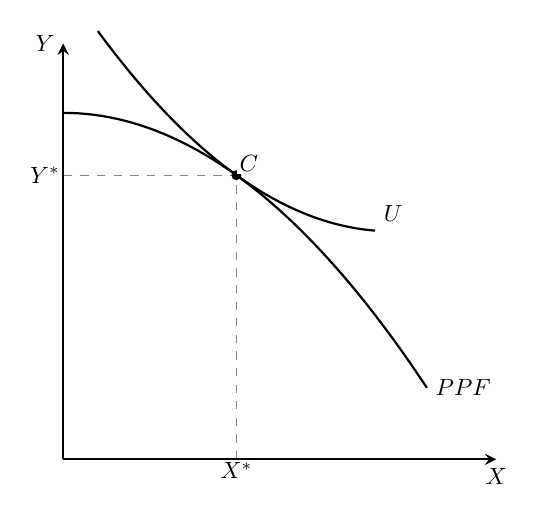
\begin{tikzpicture}[x=1.1cm, y=1.1cm, >=stealth, thick, every node/.style={scale=0.85}]
				% 1. 辅助虚线层（最底层）
				\draw[dashed, gray, thin] (2,0) -- (2,3.28) -- (0,3.28);
				
				% 2. 坐标轴
				\draw[->] (0,0) -- (5.0,0) node[below] {$X$};
				\draw[->] (0,0) -- (0,4.8) node[left] {$Y$};
				
				% 3. 供需及效用曲线（严密代数设计，切点完美相切）
				\draw[smooth, domain=0:4.2] plot (\x, {4.0 - 0.18*\x*\x}) node[right] {$PPF$};
				\draw[smooth, domain=0.4:3.6] plot (\x, {5.52 - 1.52*\x + 0.2*\x*\x}) node[above right] {$U$};
				
				% 4. 切点与标号（最高层，fill=white 防线段穿透）
				\fill (2,3.28) circle (1.8pt);
				\node[above right, fill=white, inner sep=1pt] at (2,3.28) {$C$};
				\node[below, fill=white, inner sep=1pt] at (2,0) {$X^*$};
				\node[left, fill=white, inner sep=1pt] at (0,3.28) {$Y^*$};
			\end{tikzpicture}
		\end{center}
		
		\item \textbf{为什么两个国家间的自由贸易使两国消费者的境况都得到改善？}
		
		\textbf{答：}
		在纯交换经济的环境下，自由贸易允许各方通过商品互换重新配置资源，从而移动到交换契约曲线上更具效率的配置点，实现贸易双方的互利共赢。而在包含生产的开放经济中，自由贸易则能带来更深层次的福利改善。
		
		当两国之间存在产业结构、资源禀赋或技术水平的差异时，自由贸易引导每个国家根据自身相对成本更低的领域进行专业化分工。这种国际分工打破了单一国家内部资源存量的瓶颈约束，使两国的总体消费边界得以扩展到各自孤立状态下的生产可能性边界之外，从而令两国的消费者境况同时得到改善。
		
		\item \textbf{如果国家 A 在生产两种商品上和国家 B 相比都具有绝对优势，那么国家 A 与国家 B 开展贸易就不符合 A 的利益。这种说法是对吗？试解释。}
		
		\textbf{答：}
		这种说法是错误的。国际贸易的根本基础和决定力量在于比较优势，而非绝对优势。即使一个国家在所有商品的生产效率上都表现出绝对的技术领先或较低的绝对生产成本，它也不可能在所有商品上都具备比较优势。
		
		例如国家 A 在生产两种商品上都效率更高，但其内部生产两商品的相对机会成本必定不同。国家 A 应当集中资源生产自身国内机会成本更低、即具有比较优势的商品，并与国家 B 进行国际交换。通过这种基于比较利益的专业化分工模式，两国的总产出与福利均能实现最优化，国家 A 同样可以从中获得超过孤立状态下的贸易利得。
		
		\item \textbf{你是否同意下面的陈述？试解释：\\（1）如果 3 磅奶酪可以交换 2 瓶酒，那么奶酪的价格是酒的价格的 2/3。\\（2）只有当一个国家相对于它的贸易伙伴能在较低的绝对成本水平上生产时，它才能从交易中获益。\\（3）如果生产的边际成本和平均成本固定，那么对于这个国家来说，它应该完全专业化生产一些产品，而进口其余的产品。\\（4）假设劳动力是惟一的投入，生产 1 码布的机会成本是 3 蒲式耳小麦，那么每单位小麦生产需要 3 倍于 1 单位布所需的劳动投入。}
		
		\textbf{答：}
		对于第一种陈述，表示同意。根据竞争性市场的一般均衡原理，两种商品的交换比例由其相对价格决定，由 3 磅奶酪可以交换 2 瓶酒可知其价格方程满足 $3 P_c = 2 P_w$，代数变形后即得奶酪的价格等于酒的价格的 $2/3$。
		
		对于第二种陈述，表示不同意。国际贸易的利益源泉在于两国的比较优势而非绝对优势。即使一个国家在所有商品的生产上都处于绝对的技术劣势，只要国内不同商品的相对机会成本存在差异，便能通过专业化生产并出口具有比较优势的商品来获得贸易利得。
		
		对于第三种陈述，表示同意。固定的边际成本与平均成本意味着该国的生产可能性边界在几何上表现为一条直线。在开放经济中，面对既定的国际相对价格，该线性生产边界下的社会利润最大化最优解通常表现为角点解，因而该国应当实施完全的专业化生产。
		
		对于第四种陈述，表示不同意。生产 1 码布的机会成本是 3 蒲式耳小麦，意味着在劳动投入总量固定的约束下，多生产 1 码布所消耗的劳动力资源足以生产 3 蒲式耳小麦。因此，生产 1 码布所需的劳动投入在数值上应当是生产 1 蒲式耳小麦所需劳动投入的 3 倍。
		
		\item \textbf{市场失灵的四个主要来源是什么？在每种情况下都简单解释为什么竞争性市场不能有效率地运作。}
		
		\textbf{答：}
		市场失灵是指现实中价格机制无法有效配置资源，导致社会整体福利未能达到帕累托最优的状态。其四个核心来源分别是市场势力、不完全信息、外部性以及公共物品。
		
		当市场上存在垄断等市场势力时，独占企业的边际收益曲线与平均收益曲线发生分离，导致其实现利润最大化时的均衡价格高于边际成本。此时虽然消费领域的交换依然可能有效，但社会并未能以最低的成本提供最合意的产量组合，导致产量偏离帕累托最适水平。
		
		在不完全信息的市场中，买卖双方对商品质量、要素技术等核心参数的了解存在非对称性。这种信息缺损与不对称会直接引发逆向选择和道德风险，破坏价格作为供求信号的传导效率，甚至导致大量原本可实现帕累托改进的高效交易市场直接发生萎缩或崩溃。
		
		外部性的存在则使得经济主体的私人成本与社会成本、或私人利益与社会利益发生割裂。由于自由竞争的市场体系无法提供一种自发的补偿机制让交易双方承担全部社会后果，这会导致带有外部不经济的商品供给严重过剩，而带有外部经济的商品则面临供给不足。
		
		公共物品天然具备非竞争性与非排他性。非排他性导致任何消费者都可以在不支付边际成本的情况下进行“免费搭便车”式消费，这使得私人厂商无法通过价格机制回收开发成本。自由市场的自发调节最终会使得公共物品在全社会范围内面临生产匮乏与供给中断的困境。
	\end{enumerate}
	\newpage
	\section{练习题}
	\begin{enumerate}[label=\textbf{\arabic*.}, leftmargin=*]
		\item \textbf{假定金（G）和银（S）是替代品，因为它们都是抵制通货膨胀的保值品。再假定两者的供给在短期内是固定的（ $Q_{G}=75,\ Q_{S}=300$ ），而对金和银的需求由下列方程给定：\\ $P_{G} = 975 - Q_{G} + 0.5 P_{S}$ \\ $P_{S} = 600 - Q_{S} + 0.5 P_{G}$ \\（1）金和银的均衡价格是多少？\\（2）假定新发现金矿使金的供给增加到 150。这一发现会如何影响金和银的价格？}
		
		\textbf{答：}
		为了求解黄金与白银市场的初始均衡价格，需要将短期内完全固定的两商品供给总量分别代入各自对应的市场需求方程中，从而构建双市场的一般均衡联立方程组。
		\[
		\begin{cases}
			P_G = 975 - 75 + 0.5 P_S \\
			P_S = 600 - 300 + 0.5 P_G
		\end{cases}
		\implies
		\begin{cases}
			P_G = 900 + 0.5 P_S \\
			P_S = 300 + 0.5 P_G
		\end{cases}
		\]
		
		通过将白银的价格方程代入黄金的价格方程中进行代数变形与联立求解，可以精确计算出两个贵金属市场在初始状态下的一般均衡价格。
		\[
		P_G = 900 + 0.5 (300 + 0.5 P_G) \implies 0.75 P_G = 1050
		\]
		
		解得黄金的初始均衡价格 $P_G$ 为 1400 美元，将该结果反代回白银的市场需求方程中，计算出白银的初始均衡价格 $P_S$ 为 1000 美元。
		
		当新金矿的开采导致黄金的短期市场供给量由 75 增加至 150 时，黄金市场的出清条件将发生外生改变，需要重新建立一般均衡联立方程。
		\[
		\begin{cases}
			P_G = 975 - 150 + 0.5 P_S \\
			P_S = 600 - 300 + 0.5 P_G
		\end{cases}
		\implies
		\begin{cases}
			P_G = 825 + 0.5 P_S \\
			P_S = 300 + 0.5 P_G
		\end{cases}
		\]
		
		通过代数消元法对上述新方程组进行联立求解，计算出黄金供给外生扩张后的新均衡价格组合。此时，黄金的均衡价格下降至 1300 美元，而白银由于受到替代效应的交叉反馈冲击，其均衡价格也同步联动下跌至 950 美元。
		
		\item \textbf{考虑到反馈效应，请对以下各种情形做一般均衡分析：\\（1）禽流感的爆发对于鸡肉市场和猪肉市场有什么影响？\\（2）机票征税的增加对加利福尼亚之类的主要旅游目的地，以及那些旅游地的旅馆有什么影响？}
		
		\textbf{答：}
		禽流感的爆发会导致消费者因食品安全顾虑而使其对鸡肉的需求发生剧烈萎缩。由于鸡肉与猪肉在消费上具有强替代属性，鸡肉需求曲线的左移会引致大量购买力涌入猪肉市场，引发猪肉的需求增加与市场价格飙升。
		
		而在一般均衡的框架下，猪肉价格的急速上涨会反过来通过跨市场反馈效应，重新刺激部分对价格敏感的消费者回调鸡肉消费，从而在一定程度上减缓鸡肉价格的下跌斜率。最终两个替代品市场在相互贴合反馈中达成一般均衡，鸡肉价格回落而猪肉价格上升，但波动的最终幅度均弱于局部均衡的孤立预测。
		
		对民航机票加征税收会直接抬高大众的出行总成本，导致机票需求曲线因价格攀升而向左移动。由于航空出行与目的地酒店住宿在空间上属于强互补品，访客流量的断崖式下跌将直接导致加州等旅游目的地的旅馆客房需求发生结构性萎缩，引发酒店客房价格下跌。
		
		然而目的地酒店房费的走低反过来降低了游客在当地的综合居留成本，这又会通过互补品市场的逆向反馈，在一定程度上刺激民航需求的局部回升。这种跨市场的多轮循环反馈会部分抵消由税收引发的民航初始价格跌幅，最终两个互补市场将在相对较低的产销量和均衡价格水平上达成新的一般均衡。
		
		\item \textbf{珍妮有 3 升饮料和 9 个三明治。而鲍勃有 8 升饮料和 4 个三明治。在这些禀赋下，珍妮用饮料换三明治的边际替代率是 4，而鲍勃的边际替代率是 2。画出埃奇沃思盒形图，说明这一资源配置是不是有效率的。如果是，解释原因；如果不是，那么怎样的交换会使双方的境况都得到改善呢？}
		
		\textbf{答：}
		由于珍妮和鲍勃当前的边际替代率不相等，意味着双方对商品的主观边际评价存在偏差，因此当前的资源配置未达到帕累托最优，属于无效率配置。在这种状态下，全社会存在着可以通过自愿交易来释放的潜在福利增量。
		
		由于珍妮用饮料换三明治的边际替代率大于鲍勃，说明相对于三明治而言，珍妮对饮料的边际偏好更高。此时如果珍妮用多余的三明治去交换鲍勃手中的饮料，就可以在不损害任何一方效用的前提下实现互利双赢。
		
		例如，珍妮可以用 3 个三明治向鲍勃交换 1 升饮料。对于珍妮而言，获得 1 升饮料愿意最多放弃 4 个三明治，现在只需支付 3 个，其境况得到改善；对于鲍勃而言，放弃 1 升饮料只需补偿 2 个三明治即可维持原有效用，现在得到了 3 个，其福利同样获得提升。
		
		双方可以通过这种互利交易不断调整商品配置，直至两者的无差异曲线在某点完全相切。在切点处双方的边际替代率达成一致，市场便在契约曲线上实现了帕累托最优的有效率分配。
		
		\begin{center}
			\small
			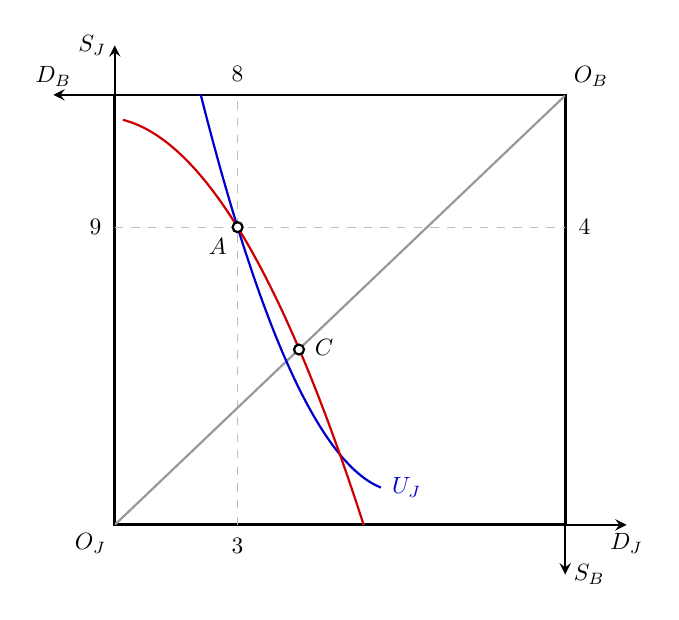
\begin{tikzpicture}[x=0.52cm, y=0.42cm, >=stealth, thick, every node/.style={scale=0.85}]
				% 1. 核心埃奇沃思闭合矩阵外框
				\draw[line width=1pt] (0,0) rectangle (11,13);
				
				% 2. 坐标轴外延射线 (适度外延，复刻标准学术风格)
				\draw[->] (0,0) -- (12.5,0) node[below] {$D_J$};
				\draw[->] (0,0) -- (0,14.5) node[left] {$S_J$};
				\draw[->] (11,13) -- (-1.5,13) node[above] {$D_B$};
				\draw[->] (11,13) -- (11,-1.5) node[right] {$S_B$};
				
				% 原点标号
				\node[below left] at (0,0) {$O_J$};
				\node[above right] at (11,13) {$O_B$};
				
				% 3. 初始禀赋分割辅助虚线
				\draw[dashed, gray!50, thin] (3,0) -- (3,13);
				\draw[dashed, gray!50, thin] (0,9) -- (11,9);
				
				% 坐标轴标签物理分离技术 (精细消除视窗重叠)
				\node[below, yshift=-2pt] at (3,0) {$3$};
				\node[left, xshift=-2pt] at (0,9) {$9$};
				\node[above, yshift=2pt] at (3,13) {$8$};
				\node[right, xshift=2pt] at (11,9) {$4$};
				
				% 4. 核心曲线绘图图层管理 (引入底层强制裁切机制，杜绝曲线溢出盒体)
				\begin{scope}
					\clip (0,0) rectangle (11,13);
					
					% 契约曲线 (直线平滑过渡，利用 sloped 自动完美旋转标签，彻底根除报错)
					\draw[smooth, domain=0:11, color=gray!80, thick] plot (\x, {1.18*\x});
					
					% 詹姆斯的无差异曲线 U_J (彻底净化非法键值，在曲线末端优雅落字)
					\draw[smooth, domain=1.0:6.5, color=blue!80!black] plot (\x, {9 + 4*(3-\x) + 0.5*(3-\x)^2})
					node[right, xshift=1pt] {$U_J$};
					
					% 布莱恩的无差异曲线 U_B
					\draw[smooth, domain=0.2:6.5, color=red!80!black] plot (\x, {9 + 2*(3-\x) - 0.3*(3-\x)^2})
					node[left, xshift=-1pt] {$U_B$};
				\end{scope}
				
				% 5. 核心均衡配置点打靶 (fill=white 擦除交叉线干扰，确保文字绝对清晰)
				% 初始禀赋点 A
				\fill[white] (3,9) circle (1.8pt); \draw (3,9) circle (1.8pt);
				\node[below left, xshift=-1pt, yshift=-1pt] at (3,9) {$A$};
				
				% 最优配置点 C (将其置于无差异曲线和契约曲线的左上方，规避重叠噪音)
				\fill[white] (4.5,5.3) circle (1.8pt); \draw (4.5,5.3) circle (1.8pt);
				\node[right, xshift=3pt, yshift=1pt] at (4.5,5.3) {$C$};
			\end{tikzpicture}
		\end{center}
		
		\item \textbf{詹妮弗和德鲁都消费橙汁和咖啡。詹妮弗以橙汁换咖啡的边际替代率为 1，德鲁以橙汁换咖啡的边际替代率等于 3。如果橙汁的价格等于 2 美元，而咖啡的价格等于 3 美元，那么哪一个市场存在超额需求？你认为这两种商品的价格会有什么变化？}
		
		\textbf{答：}
		詹妮弗与德鲁对橙汁相对咖啡的边际替代率存在显著差异，这表明当前的相对价格未能使双方同时达到消费的最优均衡。在既定的价格下，市场上橙汁与咖啡的相对价格比率为三分之二，这构成了客观的市场交换比率。
		\[
		\frac{P_o}{P_c} = \frac{2}{3}
		\]
		
		比较可知，两位消费者对橙汁的个人边际评价均严格高于市场的相对价格比率。这意味着在当前的价位下，两人均认为橙汁的主观价值被市场低估，从而表现出强烈的意愿去出售咖啡并买入橙汁。
		
		由于市场主体在决策上表现出高度的一致性，橙汁市场将会面临巨大的买方涌入，从而表现出严重的超额需求。与之相对应，咖啡市场则会由于大量抛售而呈现出超额供给。因此，橙汁的市场价格在竞争驱动下将会攀升，而咖啡的价格则会趋于下跌。
		
		\item \textbf{请填充以下表格中空缺的信息。对每一个表，根据已有的信息来确认可能的交易行为，然后确定最终的资源配置情况和相应的边际替代率值。用埃奇沃思盒形图来解释你所给出的结果。\\（1）诺曼以食物换衣服的边际替代率为 1，吉娜以食物换衣服的边际替代率为 4。\\（2）迈克尔以食物换衣服的边际替代率为 1/2，凯利以食物换衣服的边际替代率为 3。}
		
		\textbf{答：}
		对于第一种情形，诺曼与吉娜之间存在清晰的边际替代率差距。通过让吉娜向诺曼提供衣服以换取食物，可以实现帕累托改进。完成模拟填充后的分配与贸易逻辑如表格所示：
		\begin{center}
			\small
			\renewcommand{\arraystretch}{1.2}
			\setlength{\tabcolsep}{6pt}
			\begin{tabular}{cccc}
				\hline
				个人 & 初始配置 & 贸易行为 & 最终配置 \\ \hline
				诺曼 & 6F, 2C & 出售 1F 换回 3C & 5F, 5C \\
				吉娜 & 1F, 8C & 出售 3C 换回 1F & 2F, 5C \\ \hline
			\end{tabular}
		\end{center}
		
		在相对应的几何结构中，贸易起始于具有效率赤字的初始配置点。双方通过互利交换向盒子内部移动，最终驻留于无差异曲线完美相切的有效率位点。此时，两人的最终边际替代率收敛于两者初始边际替代率之间的均衡值。
		
		\begin{center}
			\small
			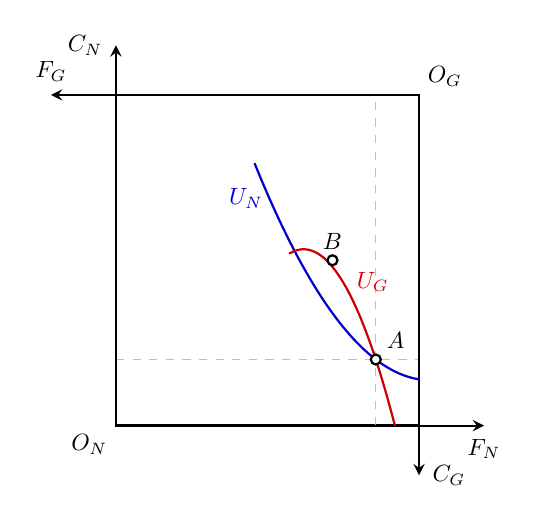
\begin{tikzpicture}[x=0.55cm, y=0.42cm, >=stealth, thick, every node/.style={scale=0.85}]
				% 1. 核心埃奇沃思闭合矩阵外框
				\draw[line width=1pt] (0,0) rectangle (7,10);
				
				% 2. 初始禀赋配置分割辅助虚线
				\draw[dashed, gray!50, thin] (6,0) -- (6,10);
				\draw[dashed, gray!50, thin] (0,2) -- (7,2);
				
				% 3. 四向反向坐标轴外延射线 (防撞击物理分离)
				\draw[->] (0,0) -- (8.5,0) node[below, yshift=-2pt] {$F_N$};
				\draw[->] (0,0) -- (0,11.5) node[left, xshift=-2pt] {$C_N$};
				\draw[->] (7,10) -- (-1.5,10) node[above, yshift=2pt] {$F_G$};
				\draw[->] (7,10) -- (7,-1.5) node[right, xshift=2pt] {$C_G$};
				
				% 原点标号定位
				\node[below left] at (0,0) {$O_N$};
				\node[above right] at (7,10) {$O_G$};
				
				% 4. 曲线独立绘图图层 (引入底层强制视窗裁切，杜绝无差异曲线外溢)
				\begin{scope}
					\clip (0,0) rectangle (7,10);
					
					% Nastya 的无差异曲线 U_N
					\draw[smooth, domain=3.2:7.0, color=blue!80!black] plot (\x, {2 - 1*(\x-6) + 0.4*(\x-6)^2});
					
					% George 的无差异曲线 U_G
					\draw[smooth, domain=4.0:6.8, color=red!80!black] plot (\x, {2 - 4*(\x-6) - 1.2*(\x-6)^2});
				\end{scope}
				
				% 5. 文本标签避让安置 (将标签内移至透镜开阔带，彻底消除边界重叠噪音)
				\node[blue!85!black, above left] at (3.6, 6.3) {$U_N$};
				\node[red!85!black, below left] at (6.5, 4.9) {$U_G$};
				
				% 6. 核心点打靶与标号 (fill=white 擦除交叉线干扰)
				% 初始禀赋点 A
				\fill[white] (6,2) circle (1.8pt); \draw (6,2) circle (1.8pt);
				\node[above right, xshift=1pt, yshift=1pt] at (6,2) {$A$};
				
				% 帕累托改进点 B
				\fill[white] (5,5) circle (1.8pt); \draw (5,5) circle (1.8pt);
				\node[above,yshift=1pt] at (5,5) {$B$};
			\end{tikzpicture}
		\end{center}
		
		对于第二种情形，迈克尔与凯利的初始主观评价同样失衡。迈克尔更偏好衣服，而凯利更偏好食物。双方通过让迈克尔转让食物给凯利来获取衣服，模拟填充后的具体贸易方案如表格所示：
		\begin{center}
			\small
			\renewcommand{\arraystretch}{1.2}
			\setlength{\tabcolsep}{6pt}
			\begin{tabular}{cccc}
				\hline
				个人 & 初始配置 & 贸易行为 & 最终配置 \\ \hline
				迈克尔 & 10F, 3C & 出售 1F 换回 1C & 9F, 4C \\
				凯利 & 5F, 15C & 出售 1C 换回 1F & 6F, 14C \\ \hline
			\end{tabular}
		\end{center}
		
		在对应的盒形图几何映射中，资源配置由于贸易而从初始失衡点向契约曲线靠拢。在最终达成的切点处，两个消费者的无差异曲线斜率绝对值完全相等，此时以食物换衣服的边际替代率稳定在双方均能接受的契合水平。
		
		\begin{center}
			\small
			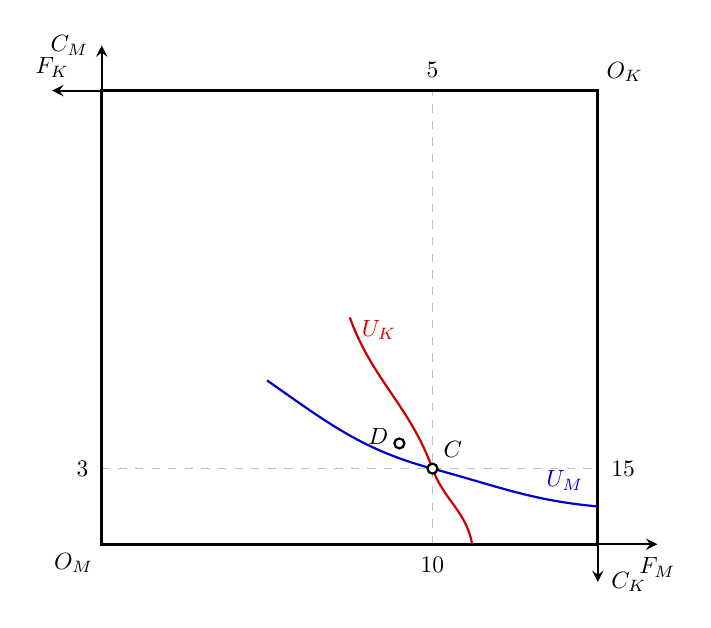
\begin{tikzpicture}[x=0.42cm, y=0.32cm, >=stealth, thick, every node/.style={scale=0.85}]
				% 1. 核心埃奇沃思闭合矩阵外框 (界定 15 * 18 的总资源边界)
				\draw[line width=1pt] (0,0) rectangle (15,18);
				
				% 2. 初始禀赋分割辅助虚线 (严格对齐 10 和 3 的切分点)
				\draw[dashed, gray!50, thin] (10,0) -- (10,18);
				\draw[dashed, gray!50, thin] (0,3) -- (15,3);
				
				% 3. 四向反向坐标轴外延射线 (复刻教科书标准学术风格)
				\draw[->] (0,0) -- (16.8,0) node[below, yshift=-2pt] {$F_M$};
				\draw[->] (0,0) -- (0,19.8) node[left, xshift=-2pt] {$C_M$};
				\draw[->] (15,18) -- (-1.5,18) node[above, yshift=2pt] {$F_K$};
				\draw[->] (15,18) -- (15,-1.5) node[right, xshift=2pt] {$C_K$};
				
				% 原点标号相对错位放置
				\node[below left] at (0,0) {$O_M$};
				\node[above right] at (15,18) {$O_K$};
				
				% 4. 坐标轴标签数理同步 (彻底修复原版点线不对应的脱节错误)
				\node[below, yshift=-2pt] at (10,0) {$10$};
				\node[left, xshift=-2pt] at (0,3) {$3$};
				\node[above, yshift=2pt] at (10,18) {$5$};
				\node[right, xshift=2pt] at (15,3) {$15$};
				
				% 5. 引入底层画布自动裁切机制，确保贝塞尔曲线绝对内敛于盒体
				\begin{scope}
					\clip (0,0) rectangle (15,18);
					
					% 麦地那的无差异曲线 U_M (平滑通过 C 点并向左上方自然拱起)
					\draw[smooth, color=blue!80!black] (5,6.5) to[out=-35, in=165] (10,3) to[out=-15, in=175] (15,1.5);
					
					% 凯伦的无差异曲线 U_K (平滑通过 C 点并向右下方自然凹陷)
					\draw[smooth, color=red!80!black] (7.5,9) to[out=-70, in=110] (10,3) to[out=-70, in=100] (11.2,0);
				\end{scope}
				
				% 6. 效用文本标签避让安置 (精准置于曲线末端开阔带，消除视觉折叠)
				\node[blue!85!black, above] at (14, 1.8) {$U_M$};
				\node[red!85!black, right] at (7.6, 8.5) {$U_K$};
				
				% 7. 核心配置点打靶 (fill=white 强力清除交叉线干扰，保证极致 scannability)
				% 初始禀赋点 C
				\fill[white] (10,3) circle (1.8pt); \draw (10,3) circle (1.8pt);
				\node[above right, xshift=1pt, yshift=1pt] at (10,3) {$C$};
				
				% 帕累托改进点 D (完美落入 U_M 与 U_K 围合而成的透镜中心)
				\fill[white] (9,4) circle (1.8pt); \draw (9,4) circle (1.8pt);
				\node[below left, xshift=-1pt, yshift=10pt] at (9,4) {$D$};
			\end{tikzpicture}
		\end{center}
		
		\item \textbf{在对两人之间交换的分析中，假定两个人的偏好完全相同，契约曲线会不会是一条直线？请解释。你能想出一个相反的例子吗？}
		
		\textbf{答：}
		如果两个消费者的偏好完全相同，且该偏好在结构上满足齐次性（即属于同质齐次偏好），那么在埃奇沃思盒形图中，连接两个对顶原点的对角直线就是两人的契约曲线。
		
		在齐次偏好的约束下，消费者的边际替代率仅取决于两种商品消费数量的相对比率，而与绝对消费规模无关。此时两人的效用扩展线均表现为从各自原点引出的一条射线。当双方的原点在盒子中对顶放置时，具有相同斜率的扩展射线将合二为一，形成一条贯穿整个盒形图的契约直线。
		\[
		MRS_{XY} = \frac{MU_x}{MU_y} = \frac{2y}{x}
		\]
		
		以相同的效用函数为例进行代数推导。将两个消费者各自面临的资源约束代入边际替代率相等的效率标准方程中，可以清晰展示其线性的几何特征。
		\[
		\frac{2y_1}{x_1} = \frac{2y_2}{x_2} \implies \frac{y_1}{x_1} = \frac{Y' - y_1}{X' - x_1} \implies y_1 = \left(\frac{Y'}{X'}\right) x_1
		\]
		
		然而，如果偏好虽然相同但并不满足齐次性条件，契约曲线就通常不会表现为一条直线。例如，当其中一种商品属于劣等品时，随着消费者收入或总财富的增加，其对该劣等品的消费量绝对值反而会缩减，这会导致消费扩展线发生明显的弯曲。偏好曲线的扭曲在对顶映射后，必然使得最终连结的效率切点轨迹脱离直线形态。
		
		\item \textbf{举例说出生产可能性边界可能不是凹的条件。}
		
		\textbf{答：}
		经典的生产可能性边界通常向右上方凸出（即对原点呈下凹形态），其经济学本质在于生产过程满足边际转换率递增规律，而这一规律往往由生产要素的边际报酬递减所驱动。
		
		然而，生产可能性边界的几何形态取决于生产函数的规模报酬特征及要素密集度。如果两个产业的生产函数均表现为规模报酬不变且要素密集度完全全同，则全社会的机会成本保持恒定，生产可能性边界将退化为一条直线。
		
		若两种商品的生产技术均呈现出显著的规模报酬递增，则随着某一商品产量的扩张，其边际生产成本反而会不断下降。此时，一种商品转换为另一种商品的边际转换率呈现递减趋势，从而导致生产可能性边界呈现向内凹陷（对原点下凸）的非凹形态。
		
		\item \textbf{一个垄断买方以低于竞争性工资的价格购买劳动。这种垄断势力的使用会导致什么样的无效率？如果这个劳动市场上的垄断买主也是产出市场上的垄断卖方，你的回答将会怎样改变？}
		
		\textbf{答：}
		在劳动力市场上，垄断买方为实现自身利润最大化，会遵循边际支出等于劳动的边际收入产出的核心原则来确立要素雇佣量。由于劳动力供给曲线向右上方倾斜，导致厂商面临的边际支出曲线严格位于供给曲线的左上方。
		\[
		ME = MRP_L
		\]
		
		这一垄断行为使得市场均衡要素雇佣量显著低于完全竞争水平，且支付给工人的均衡工资也严格低于劳动的边际收入产出。这种雇佣规模的萎缩直接造成了全社会产出效率的净损失，阻碍了劳动力资源在不同部门间的帕余托最优配置。
		
		若该买方在产出市场同时兼具垄断卖方身份，其面临的劳动边际收入产出将由边际收益而非产品价格决定。由于垄断卖方的边际收益严格小于市场相对价格，导致其劳动的边际收入产出曲线会发生全方位的向左下方平移。
		\[
		MRP_m = MR \cdot MP_L < P \cdot MP_L
		\]
		
		此时，产出市场的垄断势力与要素市场的买方垄断势力发生叠加扭曲。厂商为了维持双重垄断利润，会进一步缩减劳动力的雇佣规模，导致最终的社会产出水平出现更为剧烈的下降，加剧了整个经济系统的低效率与福利剥蚀。
		
		\begin{center}
			\small
			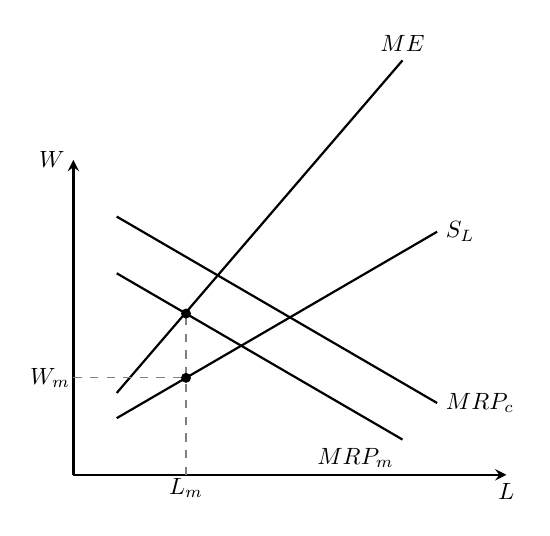
\begin{tikzpicture}[x=1.1cm, y=0.8cm, >=stealth, thick, every node/.style={scale=0.85}]
				% 1. 坐标轴
				\draw[->] (0,0) -- (5.0,0) node[below] {$L$};
				\draw[->] (0,0) -- (0,5.0) node[left] {$W$};
				
				% 2. 核心供需曲线
				\draw[domain=0.5:4.2] plot(\x, {0.8*\x + 0.5}) node[right] {$S_L$};
				\draw[domain=0.5:3.8] plot(\x, {1.6*\x + 0.5}) node[above] {$ME$};
				\draw[domain=0.5:4.2] plot(\x, {4.5 - 0.8*\x}) node[right] {$MRP_c$};
				\draw[domain=0.5:3.8] plot(\x, {3.6 - 0.8*\x}) node[below left] {$MRP_m$};
				
				% 3. 关键交点与投影
				\draw[dashed, gray, thin] (1.3,0) -- (1.3,2.56);
				\draw[dashed, gray, thin] (0,1.54) -- (1.3,1.54);
				\fill (1.3,2.56) circle (1.8pt);
				\fill (1.3,1.54) circle (1.8pt);
				
				% 4. 符号标签
				\node[below, fill=white, inner sep=1pt] at (1.3,0) {$L_m$};
				\node[left, fill=white, inner sep=1pt] at (0,1.54) {$W_m$};
			\end{tikzpicture}
		\end{center}
		
		\item \textbf{埃克米公司分别生产 $x$ 单位的 $\alpha$ 和 $y$ 单位的 $\beta$ 商品。\\（1）用生产可能性边界解释生产更多或更少的 $\alpha$ 的意愿是如何取决于 $\alpha$ 或 $\beta$ 的边际转换率的。\\（2）考虑两种极端的生产情况：①埃克米一开始生产零单位的 $\alpha$ ；②埃克米一开始生产零单位的 $\beta$ 。如果埃克米总是试图使其生产行为处在其生产可能性边界上，描述情况①和②的初始位置。当埃克米公司开始同时生产两种商品时会发生什么情况？}
		
		\textbf{答：}
		生产可能性边界代表了既定要素约束下技术有效率的产出组合空间，其几何斜率的绝对值即定义为商品 $\alpha$ 对商品 $\beta$ 的边际转换率。该指标在代数上精确测度了厂商为了多生产一单位商品 $\alpha$ 而在生产端所必须放弃的商品 $\beta$ 的机会成本。
		\[
		MRT_{\alpha\beta} = \left| \frac{\mathrm{d}\beta}{\mathrm{d}\alpha} \right| = \frac{MC_{\alpha}}{MC_{\beta}}
		\]
		
		厂商调整产出结构的微观意愿直接取决于边际转换率与外部市场相对价格比率的强弱对比。如果市场价格提供的替换比率高于生产端的机会成本，厂商就会表现出强烈的意愿缩减商品 $\beta$ 的排产，将释放的生产要素源源不断地投入到商品 $\alpha$ 的扩张中。
		
		在两种极端的边界生产环境下，如果厂商始终保持在生产可能性边界上，情况①和情况②的初始状态将完美对应于边界曲线与两个产出坐标轴的交点截距处。此时整个经济体处于完全专业化分工的角点解状态。
		
		一旦厂商打破这种单一产业垄断，开始在内部同时推进两种商品的混合生产，其配置点就会立刻脱离端点而沿着向外凸出的边界线向内移动。在边际转换率递增规律的作用下，多生产商品 $\alpha$ 所需付出的商品 $\beta$ 的代偿代价会越来越大，直至边界的切线斜率与市场价格线完全贴合。
		
		\begin{center}
			\small
			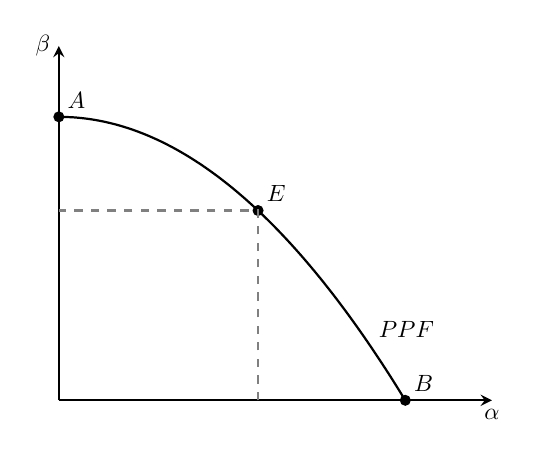
\begin{tikzpicture}[x=1.1cm, y=1.0cm, >=stealth, thick, every node/.style={scale=0.85}]
				% 坐标轴
				\draw[->] (0,0) -- (5.0,0) node[below] {$\alpha$};
				\draw[->] (0,0) -- (0,4.5) node[left] {$\beta$};
				
				% 边界曲线与端点
				\draw[smooth, domain=0:4.0] plot (\x, {3.6 - 0.225*\x*\x}) node[right,yshift=30pt,xshift=-15pt] {$PPF$};
				
				\coordinate (A) at (0,3.6);
				\coordinate (B) at (4,0);
				\coordinate (E) at (2.3,2.41);
				
				\fill (A) circle (2pt) node[above right] {$A$};
				\fill (B) circle (2pt) node[above right] {$B$};
				\fill (E) circle (2pt) node[above right] {$E$};
				
				% 切线斜率示意
				\draw[dashed, gray] (2.3,0) -- (2.3,2.41) -- (0,2.41);
			\end{tikzpicture}
		\end{center}
		
		\item \textbf{在关于生产的埃奇沃思生产盒形图的分析中，假定一种新的发明改变了食品的生产特征，从原先的规模报酬不变变为规模报酬急剧递增。请问这一变化如何影响生产契约曲线？}
		
		\textbf{答：}
		在生产的一般均衡框架中，要素契约曲线是一系列食品与衣服等产量线几何切点的连续轨迹。其代数充要条件是两个商品生产部门的边际技术替代率达到一致。
		
		如果此项新发明仅仅是单纯地改变了产出的规模效应，而没有引入要素偏向型技术变革，那么这一深化过程仅表现为等产量线在数值标签上的齐次正变换，其几何拓扑形态与切线的斜率特征将保持完全不变。由于食品部门在任何要素组合下的边际技术替代率公式均未发生任何实质性偏转，原有的切点轨迹结构将维持全同，因此要素契约曲线在坐标空间中不会发生任何位置移动。
		
		然而，如果规模报酬的急剧递增伴随着要素配置权重的调整，使得食品生产线极度依赖于某种特定要素的密集投入，等产量线的非线性几何特征就会遭到重构。此时，两个部门的边际技术替代率方程在切线配对时会发生错位，从而不可避免地驱动全社会的要素契约曲线发生明显的扭曲。
		\newpage
		\item \textbf{假设 A 国和 B 国同时生产酒和奶酪。A 国有 800 单位的劳动力，B 国有 600 单位的劳动力。在交易之前，A 国消费了 40 磅奶酪 and 8 瓶酒，而 B 国消费了 30 磅奶酪 and 10 瓶酒。}
		\begin{center}
			\small
			\renewcommand{\arraystretch}{1.2}
			\setlength{\tabcolsep}{8pt}
			\begin{tabular}{lcc}
				\hline
				& 国家 A & 国家 B \\ \hline
				每磅奶酪的劳动投入 & 10 & 10 \\
				每瓶酒的劳动投入 & 50 & 30 \\ \hline
			\end{tabular}
		\end{center}
		\textbf{（1）哪一个国家在哪一种商品的生产上具有比较优势？试解释。\\（2）请为每一个国家确定一条产出可能性曲线，用图形和代数的方法表示这条曲线。（标出交易之前的生产点 $PT$ 和交易之后的点 $P_{0}$ ）\\（3）如果两国之间的贸易为 36 磅奶酪和 9 瓶酒，标出该贸易行为之后的消费点 C。\\（4）证明两个国家都通过贸易获益了。\\（5）在贸易发生的那一点，价格线的斜率是多少？}
		
		\textbf{答：}
		通过计算各商品的机会成本可以确立两国的比较优势形态。在 A 国中，多生产 1 瓶酒需要抽取 50 单位劳动，这会导致奶酪减产 5 磅，因此 A 国酒的机会成本为 5 磅奶酪。而在 B 国中，多生产 1 瓶酒只需抽取 30 单位劳动，导致奶酪减产 3 磅，因此 B 国酒的机会成本为 3 磅奶酪。基于比较优势准则，B 国在酒的生产上具有比较优势，而 A 国在奶酪的生产上具有比较优势。
		
		将要素总量约束代入劳动投入系数中，即可确立两国各自的生产可能性边界方程。A 国的曲线方程为 $10C + 50W = 800$，化简可得 $C = 80 - 5W$；B 国的曲线方程为 $10C + 30W = 600$，化简可得 $C = 60 - 3W$。开展自由贸易后，两国的专业化分工点 $P_0$ 将分别收敛于各自具备比较优势的截距端点上。
		
		根据两国的贸易往来数量，A 国向 B 国出口 36 磅奶酪并换回 9 瓶酒。由于 A 国完全专业化生产奶酪，其产出组合为 $(0W, 80C)$，扣除出口并叠加进口后，最终消费点 $C$ 的组合为 $(9W, 44C)$。同理，完全专业化生产酒的 B 国在产出组合 $(20W, 0C)$ 的基础上进行贸易置换，其最终消费点 $C$ 的组合为 $(11W, 36C)$。
		
		通过将贸易后的消费点与贸易前的初始配置进行对比，可以直观地证明贸易利得的存在。在自由贸易体制下，A 国的消费点从原本的 $(8W, 40C)$ 提升至 $(9W, 44C)$，额外净收获 1 瓶酒和 4 磅奶酪；B 国的消费点则从 $(10W, 30C)$ 迈进至 $(11W, 36C)$，净增加 1 瓶酒和 6 磅奶酪。两国的最终消费选择均严格跨越了各自孤立状态下的实物生产极限。
		
		贸易发生时国际市场价格线的斜率即为两商品的国际交换比率。在本题的均衡框架下，36 磅奶酪可以等价交换 9 瓶酒，意味着 1 瓶酒在国际市场上可以兑换 4 磅奶酪。因此，若以酒的消费量作为横坐标、奶酪的消费量作为纵坐标，国际价格线的代数斜率在数值上严格等于 $-4$。
		
		\begin{center}
			\small
			\begin{tikzpicture}[x=0.16cm, y=0.046cm, >=stealth, thick, every node/.style={scale=0.85}]
				% ==================== 左图：国家 A ====================
				\begin{scope}
					% 1. 全局辅助虚线
					\draw[dashed, gray!50, thin] (8,0) -- (8,40) -- (0,40);
					\draw[dashed, gray!50, thin] (9,0) -- (9,44) -- (0,44);
					
					% 2. 坐标轴
					\draw[->] (0,0) -- (22,0) node[below] {$W$};
					\draw[->] (0,0) -- (0,95) node[left] {$C$};
					\node[below left] at (0,0) {$0$};
					
					% 3. 生产可能性边界 (PPF) 与世界价格线 (贸易线)
					\draw[domain=0:16, blue, thick] plot (\x, {80 - 5*\x}) node[above left,xshift=-5pt,yshift=2pt] {\scriptsize $PPF_A$};
					\draw[domain=0:19, red, dashed] plot (\x, {80 - 4*\x});
					
					% 4. 核心配置点打靶 (fill=white 强力擦除交叉线干扰)
					\fill[white] (8,40) circle (1.5pt); \draw (8,40) circle (1.5pt);
					\node[below left, xshift=-1pt] at (8,40) {$PT$};
					
					\fill[white] (9,44) circle (1.5pt); \draw (9,44) circle (1.5pt);
					\node[above right, xshift=1pt] at (9,44) {$C$};
					
					\fill[white] (0,80) circle (1.5pt); \draw (0,80) circle (1.5pt);
					\node[right, xshift=2pt] at (0,80) {$P_0$};
					
					% 5. 坐标轴标签物理分离技术 (精细防止字符视窗重叠)
					\node[below, yshift=-1pt] at (8,0) {\scriptsize 8};
					\node[below, xshift=2pt, yshift=-1pt] at (9,0) {\scriptsize 9};
					\node[left, xshift=-1pt] at (0,40) {\scriptsize 40};
					\node[left, xshift=-1pt, yshift=3pt] at (0,44) {\scriptsize 44};
					\node[left, xshift=-1pt] at (0,80) {\scriptsize 80};
					
					% 利用解耦的相对定位安置子标题
					\node[below=0.4cm] at (10,0) {(a) 国家 A};
				\end{scope}
				
				% ==================== 右图：国家 B ====================
				\begin{scope}[xshift=5cm] % 极致收紧平移间距，两图物理间距仅约0.6cm，完美防溢出
					% 1. 全局辅助虚线
					\draw[dashed, gray!50, thin] (10,0) -- (10,30) -- (0,30);
					\draw[dashed, gray!50, thin] (11,0) -- (11,36) -- (0,36);
					
					% 2. 坐标轴
					\draw[->] (0,0) -- (24,0) node[below] {$W$};
					\draw[->] (0,0) -- (0,95) node[left] {$C$};
					\node[below left] at (0,0) {$0$};
					
					% 3. 生产可能性边界 (PPF) 与世界价格线 (贸易线)
					\draw[domain=0:20, blue, thick] plot (\x, {60 - 3*\x}) node[above left,xshift=-10pt,yshift=3pt] {\scriptsize $PPF_B$};
					\draw[domain=0:19, red, dashed] plot (\x, {80 - 4*\x});
					
					% 4. 核心配置点打靶
					\fill[white] (10,30) circle (1.5pt); \draw (10,30) circle (1.5pt);
					\node[below left, xshift=-1pt] at (10,30) {$PT$};
					
					\fill[white] (11,36) circle (1.5pt); \draw (11,36) circle (1.5pt);
					\node[above right, xshift=1pt] at (11,36) {$C$};
					
					\fill[white] (20,0) circle (1.5pt); \draw (20,0) circle (1.5pt);
					\node[above right, xshift=1pt] at (20,0) {$P_0$};
					
					% 5. 坐标轴标签物理分离技术
					\node[below, yshift=-1pt] at (10,0) {\scriptsize 10};
					\node[below, xshift=2pt, yshift=-1pt] at (11,0) {\scriptsize 11};
					\node[left, xshift=-1pt] at (0,30) {\scriptsize 30};
					\node[left, xshift=-1pt, yshift=3pt] at (0,36) {\scriptsize 36};
					\node[below, yshift=-1pt] at (20,0) {\scriptsize 20};
					
					\node[below=0.4cm] at (11,0) {(b) 国家 B};
				\end{scope}
			\end{tikzpicture}
		\end{center}
		
		\item \textbf{假设一个面包店有 16 名员工，分别作为面包师（B）和蛋糕师（C），因此 B+C=16。画出以下生产函数时的生产可能性边界（y 是面包产量，x 是蛋糕产量）：\\（1） $y = 2B^{0.5}, x = C^{0.5}$ \\（2） $y = B, x = 2C^{0.5}$}
		
		\textbf{答：}
		对于第一种生产配置情形，通过将人员总量约束方程 $B = 16 - C$ 直接嵌入到面包的生产函数中，可以消除人员投入变量。随后利用蛋糕的产出方程可反导出要素需求回归式 $C = x^2$。将该式反代回面包函数中，便能顺利推导出面包与蛋糕之间的全社会生产可能性边界方程。
		\[
		y = 2(16 - C)^{0.5} \implies y = 2\left(16 - x^2\right)^{0.5}
		\]
		
		该方程在几何上属于标准的椭圆弧形态。由于两部门在技术上均面临劳动力投入的边际报酬递减，导致随着蛋糕产量的增加，其不得不剥蚀的面包产量在边缘处加速放大，从而使得最终描绘出的边界曲线呈现出经典的顺向内凹形状。
		
		对于第二种生产配置情形，同样遵循要素消元的基本步骤。由面包函数直接推知 $B = y$，而由蛋糕函数的逆运算可求得所需的蛋糕师人数满足 $C = x^2 / 4$。将这两组要素投入量同时导入到面包店的总人数限制条件中，便能求出该技术形态下的生产可能性边界方程。
		\[
		y + \frac{x^2}{4} = 16 \implies y = 16 - \frac{x^2}{4}
		\]
		
		在此类技术环境中，虽然面包部门在代数上呈现出恒定的规模报酬特性，但由于蛋糕部门内部依旧受制于劳动力边际报酬递减规律，导致多生产蛋糕的机会成本仍旧随产量扩张而递增。因此，在二维产出空间中描绘出的生产可能性边界依然表现为平滑内凹的抛物线弧段。
		
		\begin{center}
			\small
			\begin{tikzpicture}[x=0.6cm, y=0.32cm, >=stealth, thick, every node/.style={scale=0.8}]
				% 左图：方程 (1)
				\draw[->] (0,0) -- (5.2,0) node[below] {$x$};
				\draw[->] (0,0) -- (0,9.5) node[left] {$y$};
				\draw[domain=0:4, blue, thick, smooth] plot (\x, {2*sqrt(16-\x*\x)});
				\node[below] at (4,0) {\scriptsize 4};
				\node[left] at (0,8) {\scriptsize 8};
				\node[below] at (2.2,-1.5) {(a) 边界形态 (1)};
				
				% 右图：方程 (2)（高度紧凑平移，防双栏错位）
				\begin{scope}[xshift=6.5cm, x=0.32cm, y=0.16cm]
					\draw[->] (0,0) -- (9.5,0) node[below] {$x$};
					\draw[->] (0,0) -- (0,18.5) node[left] {$y$};
					\draw[domain=0:8, blue, thick, smooth] plot (\x, {16 - \x*\x/4});
					\node[below] at (8,0) {\scriptsize 8};
					\node[left] at (0,16) {\scriptsize 16};
					\node[below] at (4.5,-3.0) {(b) 边界形态 (2)};
				\end{scope}
			\end{tikzpicture}
		\end{center}
	\end{enumerate}
	
	% =======================================================
	%                 第 17 章：信息不对称的市场
	% =======================================================
	\chapter{信息不对称的市场}
	
	\section{复习题}
	\begin{enumerate}[label=\textbf{\arabic*.}, leftmargin=*]
		\item \textbf{当一个市场在其他方面都是完全竞争的时候，为什么买方和卖方之间的不对称信息会导致市场失灵？}
		
		\textbf{答：} 信息不对称是指交易双方对商品质量、成本等关键信息的掌握程度不对等。
		在完全竞争市场中，价格机制顺畅运行的前提是买卖双方均拥有完全信息。
		一旦信息出现不对称，价格将无法同时准确反映买方的边际收益与卖方的边际成本。
		这会导致低质量商品驱逐高质量商品的逆向选择，或契约签订后隐藏行动的道德风险。
		资源配置由此偏离帕累托最优状态，在极端情况下甚至会导致整个市场完全萎缩与崩溃。
		
		\item \textbf{假设旧车市场是一个“柠檬”市场。你预期售出的旧车的修理记录与没有售出的旧车的修理记录相比会怎样？}
		
		\textbf{答：} 预期在市场上成功售出的旧车，其平均修理记录将显著多于未售出的旧车。
		旧车市场是典型的信息不对称市场，卖方垄断了车辆真实质量与维修历史的信息。
		买方因无法分辨单辆车的优劣，只能根据对市场平均质量的期望来决定愿意支付的评估价格。
		高质量旧车的车主认为该平均价格远低于其车辆的内在价值，从而选择退出市场。
		低质量旧车则因能溢价售出而大量充斥市场，导致最终在市场中成交的几乎全为劣质车。
		修理记录是车辆质量的负向代理指标，劣质车的修理记录在统计上显然更加频繁。
		因此，市场中留存并成功交易的旧车修理记录，必然高于那些退出市场的优质旧车。
		
		\begin{center}
			\small
			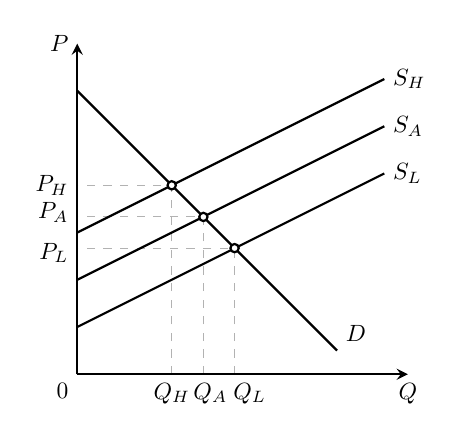
\begin{tikzpicture}[x=0.6cm, y=0.6cm, >=stealth, thick, every node/.style={scale=0.85}]
				% 1. 全局辅助虚线
				\draw[dashed, gray!60, thin] (2,0) -- (2,4) -- (0,4);
				\draw[dashed, gray!60, thin] (2.67,0) -- (2.67,3.33) -- (0,3.33);
				\draw[dashed, gray!60, thin] (3.33,0) -- (3.33,2.67) -- (0,2.67);
				
				% 坐标轴标签防重叠物理微调
				\node[left] at (0,4) {$P_H$};
				\node[left, yshift=2pt] at (0,3.33) {$P_A$};
				\node[left, yshift=-2pt] at (0,2.67) {$P_L$};
				
				\node[below] at (2,0) {$Q_H$};
				\node[below, xshift=3pt] at (2.67,0) {$Q_A$};
				\node[below, xshift=-3pt] at (3.8,0) {$Q_L$};
				
				% 2. 坐标轴
				\draw[->] (0,0) -- (7,0) node[below] {$Q$};
				\draw[->] (0,0) -- (0,7) node[left] {$P$};
				\node[below left] at (0,0) {$0$};
				
				% 3. 供需实线 (严格裁切 domain)
				\draw[domain=0:6.5, smooth, black] plot (\x, {0.5*\x + 1}) node[right] {$S_L$};
				\draw[domain=0:6.5, smooth, black] plot (\x, {0.5*\x + 2}) node[right] {$S_A$};
				\draw[domain=0:6.5, smooth, black] plot (\x, {0.5*\x + 3}) node[right] {$S_H$};
				\draw[domain=0:5.5, smooth, black] plot (\x, {-\x + 6}) node[above right] {$D$};
				
				% 4. 均衡点标号 (fill=white)
				\fill[white] (2,4) circle (1.5pt); \draw (2,4) circle (1.5pt);
				\fill[white] (2.67,3.33) circle (1.5pt); \draw (2.67,3.33) circle (1.5pt);
				\fill[white] (3.33,2.67) circle (1.5pt); \draw (3.33,2.67) circle (1.5pt);
			\end{tikzpicture}
		\end{center}
		
		\item \textbf{解释保险市场上逆向选择与道德风险的区别。其中的一种能在另一种不存在的情况下存在吗？}
		
		\textbf{答：} 逆向选择与道德风险的核心区别在于信息不对称发生的时间节点和行为性质不同。
		逆向选择发生在合同签订之前，属于隐藏信息问题，指高风险群体比低风险群体更积极地购买保险。
		这迫使保费因平均赔付率上升而提高，进而在筛选机制下将健康、低风险的投保人排挤出市场。
		
		道德风险发生在合同签订之后，属于隐藏行动问题，指投保人在获得全额保障后降低了防范动机。
		这种由激励错配引起的自私行为改变，人为调高了保险事故发生的概率及损失程度。
		这两种市场失灵机制完全独立，可以在另一方不存在的情况下单独存在。
		即使保险公司在事前拥有完全信息而消除了逆向选择，签约后投保人仍可能因规避风险成本而产生道德风险。
		
		\item \textbf{描述几种卖主能使买主相信他们的产品是高质量的方法。哪种办法适用于下列产品：梅泰洗衣机、汉堡王汉堡包、大钻石？}
		
		\textbf{答：} 卖方主要通过市场信号传递、声誉资本沉淀和产品标准化来化解买方的信任危机。
		有效的市场信号必须具备非对称成本特征，即高质量卖方的发信边际成本显著低于低质量卖方。
		常见方法包括提供长期保修承诺、树立难以复制的品牌声誉、展示专业机构的第三方认证等。
		
		针对梅泰洗衣机这类高耐用消费品，最适用的策略是提供高额的长期质量保证和保修合同。
		针对汉堡王汉堡包这类跨地域快餐，最适用的是通过标准化的特许经营维持产品品质的均质性。
		针对大钻石这类信息极其不对称的奢侈品，最适用的是出具具有法律效力的国际权威鉴定证书。
		
		\item \textbf{为什么卖主会觉得发出有关他的产品质量的信号是有利的？质量保证和保修单是如何成为市场信号的一种形式的？}
		
		\textbf{答：} 在信息不对称的柠檬市场中，若无信号传递，高质量产品将被低质量产品通过价格战驱逐。
		高质量卖方为了打破这一低价低质的逆向选择僵局，必须主动发出可信信号以实现分离均衡。
		通过成功传递信号，卖方得以向买方证明产品价值，从而获取溢价回报并扩大市场份额。
		质量保证和保修单能够成为有效的市场信号，核心在于其满足了单重合同约束的成本差异机制。
		
		低质量产品的故障率高，若提供同等力度的保修，其后期的维修与赔偿开支将呈几何级数上升。
		高质量产品由于工艺精湛，提供长期保修的边际成本极低，因而低质量企业绝无动力进行盲目效仿。
		理性消费者能够准确识别这种成本差异，从而将保修单视为高品质的可靠背书并愿意为此支付高价。
		
		\item \textbf{乔伊大学四年的时间里平均成绩很高。这是能反映乔伊的生产率高的强信号吗？为什么？}
		
		\textbf{答：} 在多数情况下，高学分绩点是一个反映高生产率的强信号。
		根据信号传递理论，优秀成绩的取得需要投入大量的时间、专注度与学习成本。
		高生产率者的学习边际成本显著低于低生产率者， Ox 从而构成了有效的分离均衡。
		它向雇主传递了乔伊具备强大学习能力、高度自律性以及快速适应新环境的特质。
		
		然而，若高校内部缺乏严谨的考核标准，该信号的有效性将会大幅减弱。
		如果乔伊是通过大量选修给分宽松的简单课程，或由考核不严的教授授课来获取高分。
		此时不同生产率个体的发信边际成本差额将不复存在，导致该成绩无法有效区分其实际能力。
		
		\item \textbf{为什么企业经理或许会实现不同于企业股东利润最大化的目标？}
		
		\textbf{答：} 现代企业中所有权与控制权的分离，导致了经理与股东之间目标函数的不一致。
		股东追求的是企业长期利润或股权价值的最大化，而经理则倾向于追求自身效用最大化。
		经理的个人目标通常包含更高的薪酬福利、更大的行政权力、职业安全感以及企业规模的扩张。
		
		信息不对称与高昂的监督成本，为经理背离股东目标提供了客观空间。
		经理处于企业运营的第一线，掌握着关于成本、市场与决策细节的绝对内部信息。
		由于股东无法无成本地精确观察经理的努力程度，委托代理问题随即产生。
		在内部控制不完善时，经理便有能力在不严重损害企业生存的前提下，牺牲部分利润以实现私利。
		
		\item \textbf{委托—代理模型如何被用来解释为什么像邮电局之类的公共企业可能追求的不是利润最大化的目标？}
		
		\textbf{答：} 公共企业的委托代理链条比私人企业更为冗长且复杂。
		公共企业的名义委托人是全体公众或政府官员，而代理人则是企业的具体经营管理者。
		政府官员本身也面临自身的效用激励，往往缺乏像私人股东那样精细监督代理人的经济动机。
		
		公共企业内部的严重信息不对称，企图赋予经理极大的自由裁量权。
		经理对企业的真实成本结构、技术细节和市场实际需求的了解远超监管官员。
		这种信息优势与缺乏硬预算约束的特性相结合，使得经理能够轻松隐瞒真实利润。
		他们倾向于将潜在利润转化为部门预算扩张、冗员配置、工作安逸度或对特定消费群体的过度补贴。
		
		\item \textbf{为什么奖金和利润分享支付计划可能解决委托—代理问题，而固定的工资支付却不能？}
		
		\textbf{答：} 解决委托代理问题的核心在于设计出满足激励相容约束的薪酬机制。
		固定工资支付将经理的个人收益与企业的经营绩效完全脱钩。
		在固定薪酬下，经理付出努力的边际收益为零，而规避努力的偷懒行为却能带来正向效用。
		这必然导致经理在信息不对称的保护下选择偷懒，使委托代理问题进一步恶化。
		
		奖金与利润分享计划则将经理的经济报酬与企业的最终产出或利润直接挂钩。
		这种机制将企业运营的部分风险分摊给经理，使双方的目标函数在边际上趋于一致。
		经理为了最大化自身的分成收益，必须选择付出高水平的努力。
		这有效克服了因无法直接监督而带来的道德风险，实现了次优的激励效果。
		
		\item \textbf{什么是效率工资？为什么当工人对他们的生产率比厂商有更多的信息时，支付效率工资对厂商是有利的？}
		
		\textbf{答：} 效率工资是指企业主动支付给员工的、显著高于市场出清水平的激励性工资。
		其核心机理是通过提高员工的偷懒成本，来提高劳动生产率并降低管理监督成本。
		
		当工人对自身生产率和努力程度拥有信息优势时，厂商往往面临严重的偷懒风险。
		由于直接监督工人的日常行为成本高昂且不完全，固定市场工资无法有效约束工人的隐藏行动。
		支付效率工资大幅提高了工人的失业惩罚代价，因为一旦偷懒被解雇，工人将面临严重的收入损失。
		这种由高工资带来的失业威胁转化为强大的自律动机，促使工人主动保持高生产率。
		同时，高工资还能在事前吸引更多高素质求职者，从而缓解了劳动力市场上的逆向选择问题。
	\end{enumerate}
	\newpage
	\section{练习题}
	\begin{enumerate}[label=\textbf{\arabic*.}, leftmargin=*]
		\item \textbf{许多消费者把著名品牌的名称看作是质量的信号，并愿为名牌产品多付钱（例如，拜尔阿斯匹林而不是一般的阿斯匹林，或者伯兹·阿艾蔬菜而不是超级市场自己牌子的蔬菜）。品牌名称能不能提供有用的质量信号？为什么？}
		
		\textbf{答：} 品牌名称能够提供非常有用的质量信号。
		建立卓越的品牌声誉需要厂商在前期广告、技术研发和渠道建设上投入高昂的沉淀成本。
		低质量产品的生产商若盲目效仿，将因极高的产品退换率和声誉折损而承担更高的边际发信成本。
		因此，只有高质量厂商才有动力锁定这一沉淀投资，消费者据此可将品牌视为甄别质量的可靠依据。
		同时，知名品牌往往伴随着严格的产品标准化流程，能有效消除新进入者带来的质量不确定性。
		
		\item \textbf{加里是毕业不久的大学生。在新的工作岗位上干了6个月之后，他最终存够了钱买他的第一辆车。
			（1）加里对轿车的式样和型号之间的区别知道得很少。他如何利用市场信号、声誉或标准化来进行比较？
			（2）你是一家银行的贷款员。在选好了一辆车之后，加里到你这里来寻求贷款。由于他毕业不久，没有较长的信贷史。尽管如此，该银行具有为新毕业生融资买车的悠久历史。这一信息在加里的例子中是否有用？如果是的，怎样有用？}
		
		\textbf{答：} （1）加里可以通过多维度的市场信息机制来化解买方的决策劣势。
		在新车市场，他可以关注厂商提供的标准化保修合同，这是对车辆内在品质的强信号。
		若选择二手车市场，他应优先选择具有高度品牌声誉的连锁经销商，其声誉资本可对车况提供背书。
		对于缺乏声誉和保修的个人车主，加里则需借助第三方专业技术检测来重塑信息的对称性。
		
		（2）该银行积累的历史贷款数据在审查加里的贷款时具有极高的统计学筛选价值。
		在缺乏个人长信贷历史的情况下，银行业已形成的“新毕业生贷款群体声誉”成为一种替代性信号。
		这一悠久历史形成的数据集，能够让贷款员有效评估该特定群体的平均违约概率与潜在偿债能力。
		银行据此可将加里归类至风险可控的细分市场并给予融资支持，从而大幅降低了因信息不对称导致的信贷配给概率。
		
		\item \textbf{一家重点大学禁止给 D 或 F 的成绩。它对自己的行动辩解说，学生在没有因不及格而退学的压力时，他们的表现会超过平均水平。该大学说，它希望所有的学生都得到 A 和 B。如果目标是把总体成绩提高到 B 或以上的水平，这是不是一项好的政策？结合道德风险问题进行讨论。}
		
		\textbf{答：} 从经济学激励逻辑来看，这是一项注定会引发严重道德风险的错误政策。
		禁止给低分在本质上割裂了学生的学习努力与绩效惩罚之间的因果反馈。
		当不及格的下限风险被校方人为移除后，学生付出学习努力的边际成本相对上升，而偷懒的边际机会成本降为零。
		这会导致原本处于及格线边缘的学生产生隐藏行动，降低日常时间投入，引发普遍的隐性偷懒行为。
		该政策不仅无法将整体能力提升至优秀水平，反而会因激励兼容机制的丧失导致教育质量的整体滑坡。
		
		\item \textbf{琼斯教授刚被一家重点大学的经济学系聘用。董事会主席刚刚声明，该大学要为本科生提供最高质量的教育。开学两个月后，琼斯教授还没有在教室讲课。看来他把所有的时间都用于经济学研究而不是教学。琼斯教授争辩说，他的研究会给系里和大学带来更多的声誉。应当允许他继续只搞研究吗？结合委托—代理问题进行讨论。}
		
		\textbf{答：} 大学与教授之间构成了典型的多任务委托代理关系，不应允许其完全脱离教学。
		大学作为委托人，其目标函数包含教学与科研双重任务；教授作为代理人，则在两项任务间分配个人精力。
		由于科研成果的社会能见度高且更易于进行定量化测度，其边际回报对教授个人而言显著高于教学。
		若大学对此不加约束，教授必然会将全部资源向科研倾斜，导致教学质量这一难以短期测度的任务被完全边缘化。
		校方应重建激励相容的契约架构，实行分类定级薪酬或将基础教学工作量作为获取科研奖金的硬性门槛。
		
		\item \textbf{面对生产的轿车有修理记录很差的名声，一些美国汽车公司为买主提供广泛的保修服务（例如，对所有零部件和与机械问题有关的修理给予七年的保修）。
			（1）根据你对柠檬市场的知识，为什么这是一项合理的政策？
			（2）这一政策是否会产生道德风险问题？请解释。}
		
		\textbf{答：} （1）这是一项通过高成本信号传递破解柠檬市场逆向选择僵局的理性决策。
		在消费者对美系车持有劣质预期时，企业必须通过非对称的保修成本向市场证明质量的真实改善。
		由于劣质车的潜在故障率高，若盲目提供长期全包保修，其后期的实际赔付成本将彻底吞噬企业利润。
		只有真正提升了制造工艺的高质量车企，才能承受长达七年的全包保修边际成本。
		这一排他性成本差额形成了有效的分离均衡，成功向消费者传递了车辆品质提升的信任信号。
		
		（2）该保修政策在契约签订后必然会诱发严重的道德风险问题。
		当车主获得了涵盖所有零部件和人工费用的长达七年的全额保障后，其承担的车辆损坏边际成本降为零。
		这会极大地削弱车主进行日常精心保养、定期维护以及规范驾驶的内在激励。
		投保人隐藏的粗暴驾驶或疏于防范等行动，将导致车辆的实际故障率和维修开支显著上升，造成福利损失。
		
		\item \textbf{为了促进竞争和提高消费者的福利，联邦贸易委员会要求厂商真实地做广告。广告的真实性如何促进竞争？为什么如果厂商做欺骗性的广告，市场的竞争性会降低？}
		
		\textbf{答：} 真实广告能够有效降低消费者的信息搜寻成本，提升市场信息透明度。
		消费者得以在不同品牌的价格与真实质量之间进行理性横向对比，从而强化了效率优胜劣汰的竞争机制。
		
		相反，欺骗性广告会严重扭曲市场信号，导致消费者无法对产品真实性价比做出准确评估。
		面对质量的不确定性，买方会产生防御性心理，倾向于长期锁死在已经验证的少数成熟大牌上。
		这不仅压制了现有厂商之间的价格竞争，还对高质新厂商构成了极高的声誉壁垒与市场准入障碍。
		
		\item \textbf{一家保险公司在考虑发行三种火灾保险单：（1）完全赔偿的保险；（2）扣除10000美元以后，超出部分完全赔偿；（3）对于所有损失给予 $90\%$ 的赔偿。哪一种保险单更可能产生道德风险问题？}
		
		\textbf{答：} 完全赔偿的保险单最可能产生严重的道德风险问题。
		道德风险源于隐藏行动的不对称性，投保人会在签约后降低其防范火灾的努力程度。
		在完全赔偿契约下，火灾发生带来的全部边际经济损失均由保险公司承担，投保人的边际受损成本为零。
		这导致其彻底失去了定期维护电路、安装消防预警装置等防范风险的主动激励。
		而后两种方案通过设置免赔额或按比例共担损失，使投保人仍需承担实质性的边际惩罚，从而有效保留了防范动机。
		
		\item \textbf{你已经看到，随着低质量产品把高质量产品逐出市场，不对称信息是如何降低市场上出售的产品的平均质量的。对于那些不对称信息盛行的市场，你是否同意下列每一种情况？简要地解释。
			（1）政府应当对消费者投诉给予补贴。
			（2）政府应当实施质量标准，例如，不应当允许厂商出售低质量产品。
			（3）高质量产品的生产者可能想提供内容广泛的保修单。
			（4）政府应当要求所有的厂商提供内容广泛的保修单。}
		
		\textbf{答：} （1）不同意。财政补贴消费者投诉会引发严重的逆向选择与道德风险。
		该补贴会诱使原本掌握充分信息的消费者故意制造虚假诉求，甚至促使劣质企业雇佣消费者恶意抹黑竞争对手。
		政府在面对巨大案卷时的甄别与监督成本极高，这类高噪信息反而会进一步加剧市场的信息不对称。
		
		（2）不同意。强制一刀切的质量标准会剥夺低端细分市场的存在合理性。
		只要低质量产品定价足够低廉且明码标价，其在边际上依然能有效匹配低收入群体的特定消费福利。
		此外，行政层面的合规检测与司法纠纷裁决，将给财政和企业带来极为沉重的社会监督负担。
		
		（3）同意。这是市场主体自发化解柠檬市场僵局、社会总成本最低的分离均衡方案。
		高质量生产者能够凭借低故障率，以极低的边际成本提供广泛的保修承诺。
		低质量厂商则因无法承受高昂的实际维修开支而放弃效仿，保修单由此成为天然、可信的质量甄别工具。
		
		（4）不同意。若政府强制所有企业提供相同力度的保修，将导致市场信号机制彻底失效。
		这把原本可以实现分离均衡的排他性发信工具强行扭曲为混同均衡，消费者将无法通过保修单鉴别品质优劣。
		同时，这也粗暴阻断了低质产品通过放弃保修来维持低价竞争优势的正常商业逻辑。
		
		\item \textbf{两家旧车行在一条大路旁并排竞争。第一家是哈里车行，它出售经过仔细检查并在必要时进行修理的高质量轿车。哈里平均要花 8000 美元购买和修理它出售的每一辆车。第二家是刘氏车行，它出售低质量轿车。刘氏车行出售的车平均每辆的成本只有 5000 美元。如果消费者知道他们所买轿车的质量，他们会很高兴地以平均每辆 10000 美元购买哈里车行出售的车，并仅以平均每辆 7000美元购买刘氏车行出售的车。}
		
		\textbf{如果没有更多的信息，消费者并不知道每家车行的轿车质量。在每家车行购车的消费者估计，不管他们到哪一家车行去，他们买到一辆高质量车的机会是相等的，因而他们愿意以平均每辆 8500 美元买车。}
		
		\textbf{哈里车行有了一个主意——它将为所有它所出售的轿车提供相应的保证书。它知道，一项期限为 $\gamma$ 年的保证书会使它平均花费 $500\gamma$ 美元，并且它还知道，如果刘氏也提供同样的保证书，那会使刘氏平均花费 $1000\gamma$ 美元。}
		
		\textbf{（1）如果哈里车行对所有出售的轿车提供一年的保修：[i] 如果刘氏车行不提供一年保修，其利润为多少？如果刘氏也提供呢？[ii] 如果刘氏车行不提供一年的保修，哈里的利润是多少？如果刘氏也提供呢？[iii] 刘氏会跟哈里一样提供一年的保修吗？[iv] 哈里提供一年的保修，这是一个好主意吗？}
		
		\textbf{（2）如果哈里车行对它的车提供两年的保修会怎样呢？这会产生可信的质量信号吗？三年的保修又会怎样呢？}
		
		\textbf{（3）如果你为哈里车行做广告，你会鼓动它提供多长时间的保修？解释原因。}
		
		\textbf{答：} （1）[i] 若刘氏不提供保修，市场实现分离，刘氏以低质价 7000 美元售车，利润为 $7000 - 5000 = 2000$ 美元。若刘氏选择盲目模仿哈里提供一年保修，市场将陷入混同状态，消费者愿意支付混同均价 8500 美元，此时刘氏的利润变为 $8500 - 5000 - 1000 \times 1 = 2500$ 美元。
		
		[ii] 若刘氏不提供保修而哈里独立提供，哈里成功获取高质量溢价，其利润为 $10000 - 8000 - 500 \times 1 = 1500$ 美元。若刘氏跟进保修导致混同，哈里的产品无法被识别，其利润退化为 $8500 - 8000 - 500 \times 1 = 0$ 美元。
		
		[iii] 刘氏车行显然会选择跟进并提供一年的保修。因为模仿行为能让刘氏的经营利润从 2000 美元提升至 2500 美元，搭便车行为在经济学上是完全理性的。
		
		[iv] 综上所述，哈里提供一年保修绝非一个好主意。因为对手的理性策略是选择模仿，这会迫使博弈收敛于糟糕的混同均衡，最终导致哈里的发信利润被完全剥蚀至零。
		
		（2）当保修期延长至两年时，若刘氏强行模仿，其利润将大幅萎缩至 $8500 - 5000 - 1000 \times 2 = 1500$ 美元。由于该收益低于其放弃发信时的诚实利润 2000 美元，刘氏将失去模仿动机。市场由此达成完美的风险分离均衡，哈里成功向市场传递了高质量的真实信号，并获取 $10000 - 8000 - 500 \times 2 = 1000$ 美元的净利润。
		
		若保修期盲目延长至三年，哈里在分离均衡下的利润将进一步缩减至 $10000 - 8000 - 500 \times 3 = 500$ 美元。由于该利润已退化到与不发出任何信号时的原始混同利润完全相等，哈里在边际上将失去继续延长保修期的经济动力。
		
		（3）在广告策划中，应当鼓动哈里车行提供精准为 1.5 年的保修期限。为了成功阻断低质对手的伪造企图，保修期 $t$ 的设定必须满足刘氏车行的激励相容约束，即模仿收益不得超过其诚实收益。
		\[
		\begin{aligned}
			8500 - 5000 - 1000t &\le 7000 - 5000 \\
			3500 - 1000t &\le 2000 \\
			1000t &\ge 1500 \implies t \ge 1.5
		\end{aligned}
		\]
		当保修期精确设定为 1.5 年时，刘氏车行模仿的边际净收益刚好归零，从而被迫退出信号市场的竞争。这不仅能以最低的发信成本建立起坚固的高质量隔离防线，还能最大化哈里车行自身的利润留存。
		
		\item \textbf{作为行业董事会的主席，你估计你的年度利润如下表所示。利润（$\pi$）取决于市场需求和你新任 CEO 的努力水平。每种需求情况发生的可能性也如下表所示。}
		
		\begin{center}
			\small
			\renewcommand{\arraystretch}{1.3}
			\setlength{\tabcolsep}{6pt}
			\begin{tabular}{lccc}
				\hline
				市场需求 & 低需求 & 中等需求 & 高需求 \\ \hline
				概率 & 0.3 & 0.4 & 0.3 \\
				低努力 & $\pi = 500$ 万美元 & $\pi = 1000$ 万美元 & $\pi = 1500$ 万美元 \\
				高努力 & $\pi = 1000$ 万美元 & $\pi = 1500$ 万美元 & $\pi = 1700$ 万美元 \\ \hline
			\end{tabular}
		\end{center}
		
		\textbf{你必须设计一个酬金计划能够最大化企业的预期利润。如果企业是风险中性的，CEO 是风险规避的，CEO 的效用函数为：当不努力时，效用 $= W^{0.5}$；当努力时，效用 $= W^{0.5} - 100$。式中，W 为 CEO 的收入（-100 是 CEO 努力的效用成本）。你知道 CEO 的效用函数，并且你和 CEO 都知道上表所示的信息。但是你不知道 CEO 的努力程度或者准确的市场需求。当然，你知道企业的利润。在以下三种薪酬制度下，你宁愿选择哪一种？为什么？第一种，支付 CEO 固定工资，575000 美元/年；第二种，支付 CEO 企业年利润的 6\%；第三种，支付 CEO 固定工资 500000 美元/年，加上当企业利润超过 1500 万美元后超出部分的 50\%。}
		
		\textbf{答：} 董事会应选择第三种薪酬制度。考核该类问题的标准方法是首先对比不同激励下首席执行官的期望效用，确定其占优努力水平，进而计算公司的最大化净期望利润。
		
		在第一种固定工资制度下，首席执行官的报酬与企业经营业绩完全脱钩。
		由于付出努力会带来固定的负效用成本，其在不同努力水平下的期望效用对比如下：
		\[
		\begin{aligned}
			E(U_L) &= 575000^{0.5} \approx 758.29 \\
			E(U_H) &= 575000^{0.5} - 100 \approx 658.29
		\end{aligned}
		\]
		显然，首席执行官将理性选择不努力。此时公司的期望净利润为：
		\[
		E(\pi_1) = 0.3 \times 500 + 0.4 \times 1000 + 0.3 \times 1500 - 57.5 = 942.5 \text{（万美元）}
		\]
		
		在第二种按比例分成制度下，首席执行官的收入为总利润的 6\%。
		将其总利润转化为美元单位后，首席执行官在两种努力水平下的期望效用分别为：
		\[
		\begin{aligned}
			E(U_L) &= 0.3 \times \sqrt{300000} + 0.4 \times \sqrt{600000} + 0.3 \times \sqrt{900000} \approx 758.76 \\
			E(U_H) &= 0.3 \times \sqrt{600000} + 0.4 \times \sqrt{900000} + 0.3 \times \sqrt{1020000} - 100 \approx 814.84
		\end{aligned}
		\]
		由于高努力的期望效用更高，该机制成功促使首席执行官选择高努力。此时公司的期望净利润为：
		\[
		E(\pi_2) = (1 - 0.06) \times (0.3 \times 1000 + 0.4 \times 1500 + 0.3 \times 1700) = 1325.4 \text{（万美元）}
		\]
		
		在第三种基本工资加超额奖金的制度下，只有在高需求且高努力时企业利润才会跨越 1500 万美元的门槛。
		此时首席执行官在不同努力水平下的期望效用对比如下：
		\[
		\begin{aligned}
			E(U_L) &= \sqrt{500000} \approx 707.11 \\
			E(U_H) &= 0.7 \times \sqrt{500000} + 0.3 \times \sqrt{500000 + 2000000 \times 0.5} - 100 \approx 762.40
		\end{aligned}
		\]
		此制度同样能诱导首席执行官选择高努力。此时公司的期望净利润为：
		\[
		E(\pi_3) = 0.3 \times (1000 - 50) + 0.4 \times (1500 - 50) + 0.3 \times (1700 - 50 - 100) = 1330 \text{（万美元）}
		\]
		
		\item \textbf{一家厂商的短期收益为 $R = 10e - e^2$。其中 $e$ 为一个典型工人（所有工人都假设为是完全一样的）的努力水平。工人选择他的收入减去努力以后的净工资 $\omega - e$（努力的单位成本假设为1）最大化的努力水平。根据下列每种工资安排，确定努力水平和利润水平（收入减去支付的工资）。解释为什么这些不同的委托—代理关系产生不同的结果。
			（1）对于 $e \geq 1$，w = 2；否则 w = 0。
			（2）$w = R / 2$。
			（3）w = R - 12.5。}
		
		\textbf{答：} （1）在这种惩罚性固定工资契约下，工人的净工资函数表现为分段形式。
		当努力水平达到边界时，工人获取最大化净收益：
		\[
		w_n = \begin{cases} 2 - e, & e \ge 1 \\ -e, & e < 1 \end{cases}
		\]
		理性工人只需满足最低合规要求，即选择最低努力水平 $e = 1$。此时厂商获得的最终利润为：
		\[
		\pi = 10 \times 1 - 1^2 - 2 = 7
		\]
		该模式由于缺乏超额边际激励，工人毫无增加努力的动力，因而无法实现更高的生产效率。
		
		（2）在比例分成契约下，工人的收益与厂商的整体产出相挂钩。
		此时工人的目标函数转化为关于努力水平的二次函数：
		\[
		w_n = \frac{1}{2}(10e - e^2) - e = 4e - 0.5e^2
		\]
		根据利润最大化的一阶条件，令导数为零即可解得工人的最优努力水平：
		\[
		\frac{dw_n}{de} = 4 - e = 0 \implies e = 4
		\]
		此时厂商享有一半的剩余收益，其最终斩获的利润水平为：
		\[
		\pi = \frac{1}{2} R = 5 \times 4 - 0.5 \times 4^2 = 12
		\]
		此项设计使得工人与厂商利益共沾，引致工人自发提高努力程度，促使厂商利润实现明显增长。
		
		（3）在固定租金契约下，工人支付完固定留存基数后成为在边际上承担完全风险的剩余索取者。
		工人的净工资目标函数可以写为：
		\[
		w_n = (10e - e^2) - 12.5 - e = 9e - e^2 - 12.5
		\]
		根据一阶优化条件进行推导，能够直接锁定工人的最优努力供给水平：
		\[
		\frac{dw_n}{de} = 9 - 2e = 0 \implies e = 4.5
		\]
		此时厂商固定的资产出租净利润即为扣除了努力激励成本后的固定数额：
		\[
		\pi = R - (R - 12.5) = 12.5
		\]
		这一关系彻底消除了边际扭曲，工人释放出最高的努力水平，从而帮助委托人锁定了最大化的确定性收益。
		\newpage
		\item \textbf{全球储贷银行有 1000 美元可以贷出。无风险的贷款在未来一年会得到 4\% 的利率。有 20\% 的违约风险（收不回来）和 80\% 履约可能的贷款利率为 30\%。
			（1）此贷款机构预期可以赚多少钱？证明无论进行有风险放贷还是进行无风险放贷，预期回报相同。
			（2）现在，假设此贷款机构知道政府将为机构做保险人，如果违约就补偿给它1000美元的本金。贷款机构会如何选择呢？政府的预期成本是多少？
			（3）假设此贷款机构不确知是否有政府担保，但会有概率 P 发生。在 P 为多少的时候，该贷款机构会选择风险性贷款呢？}
		
		\textbf{答：} （1）无风险放贷的利息回报为确定的 40 美元。
		而在风险放贷模式下，若借款人违约，银行将面临损失全部本金 1000 美元的系统性风险。
		此时高风险放贷项目的数学期望回报为：
		\[
		\begin{aligned}
			E(\pi_{\text{无风险}}) &= 1000 \times 4\% = 40 \text{（美元）} \\
			E(\pi_{\text{风险}}) &= 0.8 \times (1000 \times 30\%) + 0.2 \times (-1000) = 40 \text{（美元）}
		\end{aligned}
		\]
		精算结果表明，在完全竞争的市场出清状态下，两种资产放贷模式的预期回报完全相同。
		
		（2）当政府承诺全额承担违约本金后，高风险贷款的下行风险被彻底向外转嫁。
		此时银行面对风险放贷的预期回报函数将发生根本性扭曲：
		\[
		E(\pi_{\text{风险}}) = 0.8 \times 300 + 0.2 \times 0 = 240 \text{（美元）}
		\]
		由于 240 美元远超无风险收益的 40 美元，银行将毫无疑问地全面转向高风险放贷。
		此时政府作为事实上的兜底者，其面临的政策预期期望履约成本为：
		\[
		E(\text{成本}) = 0.8 \times 0 + 0.2 \times 1000 = 200 \text{（美元）}
		\]
		
		（3）若政府兜底行为具有不确定性，银行将基于混合概率预期来做出最终的信贷决策。
		在政府担保概率为 $P$ 的条件下，进行有风险贷款的综合期望净收益为：
		\[
		E(\pi_{\text{风险}}) = 240P + 40(1 - P) = 40 + 200P
		\]
		根据理性机构的风险决策临界条件，只要风险放贷的收益期望略微高出无风险回报即可：
		\[
		40 + 200P > 40 \implies P > 0
		\]
		这有力地论证了道德风险的极高敏感性，即只要市场上存在一丝政府救市的预期，就会诱发信贷机构非理性的过度风险扩张。
	\end{enumerate}
	
	% =======================================================
	%                 第 18 章：外部性与公共物品
	% =======================================================
	\chapter{外部性与公共物品}
	
	\section{复习题}
	\begin{enumerate}[label=\textbf{\arabic*.}, leftmargin=*]
		\item \textbf{下列哪种情形描述了外部性，哪个没有？解释它们的区别。
			（1）巴西限制咖啡出口的政策导致美国咖啡的价格上升，它反过来又导致茶叶的价格上升。
			（2）一则广告传单使一个驾驶汽车的人分心，结果使他撞上一根电线杆。}
		
		\textbf{答：} （1）此情形未构成经济学意义上的外部性。
		巴西限制咖啡出口导致美国咖啡供给减少、价格抬升，进而促使作为替代品的茶叶需求增加并涨价。
		这一连锁反应完全是通过市场价格机制的变动来传导的，属于典型的金钱外部性，并未破坏市场效率。
		
		（2）此情形构成了典型的负外部性。
		广告公司在筹划传单时，并未向社会支付因散落传单分散驾驶员注意力而引发的潜在交通事故成本。
		该行为导致私人成本与社会成本发生背离，传单对无辜的第三方造成了实质性的安全损害。
		两者的核心区别在于，前者依托价格体系实现资源重新配置，而后者在市场机制之外直接对他人施加了无法补偿的成本。
		
		\item \textbf{在减污的成本和收益不确定时，比较和对照下列三种对付污染外部性的机制：(a) 排污费；(b) 排污标准；(c) 可转让排污许可证制度。}
		
		\textbf{答：} 排污费属于价格规制，排污标准属于数量控制，而可转让排污许可证则是将两者优势兼容并蓄的市场化创新。
		在完全信息状态下，通过对排污行为征收合理的排污费，能够以最低的社会总成本促使所有厂商实现有效率的减污水平，其表现优于一刀切的法定排污标准。
		
		在减污成本与收益不确定（即信息不完全）时，机制的选择取决于边际社会成本与边际减污成本曲线的相对斜率。
		若边际社会成本曲线十分陡峭，而边际减污成本曲线相对平坦，此时数量控制性质的排污标准将显著优于排污费。
		如下图所示，若将有效率的排污费误降为 7 美元，厂商为了追求私人边际收益，会将排放量大幅扩张至 11 单位。
		由于边际社会成本极高，这在产量过剩区间引致了巨大的无谓损失，其几何面积表现为大三角形 $ABC$。
		
		相反，在此情形下若采用排污标准，即使由于信息限制将标准错误地从 8 单位放宽至 9 单位。
		其所造成的社会净损失仅为小三角形 $ADE$ 的面积，其带来的福利折损远小于收费错误带来的大三角形 $ABC$。
		可转让排污许可证兼具标准的总量可控性与费用的动态调配效率，管理机构只需锁定总许可证额度，便能确保污染总量不超标，同时利用二级市场自由交易实现最低社会减污成本。
		
		\begin{center}
			\small
			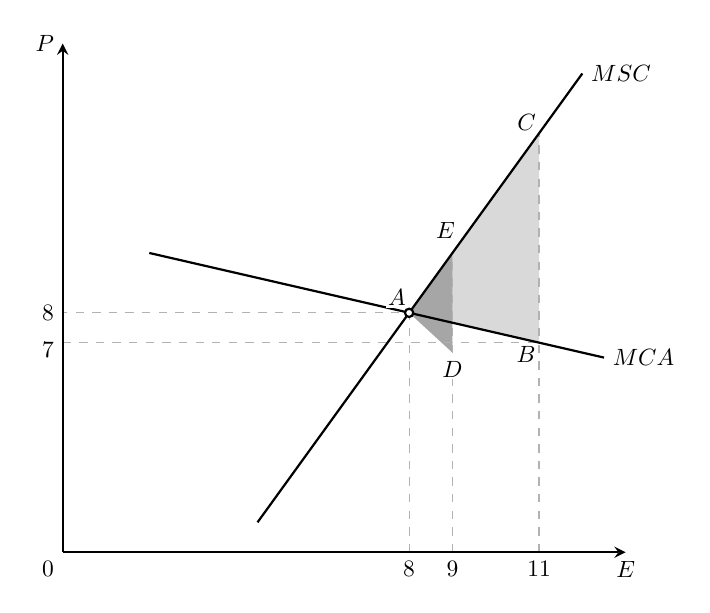
\begin{tikzpicture}[x=0.55cm, y=0.38cm, >=stealth, thick, every node/.style={scale=0.85}]
				% 1. 福利剩余区域填充 (最底层)
				\fill[gray!30] (8,8) -- (11,7) -- (11,14) -- cycle; % 三角形 ABC
				\fill[gray!70] (8,8) -- (9,6.67) -- (9,10) -- cycle; % 三角形 ADE
				
				% 2. 全局辅助虚线
				\draw[dashed, gray!60, thin] (8,0) -- (8,8) -- (0,8);
				\draw[dashed, gray!60, thin] (9,0) -- (9,10);
				\draw[dashed, gray!60, thin] (11,0) -- (11,14);
				\draw[dashed, gray!60, thin] (0,7) -- (11,7);
				
				% 坐标轴标签物理分离防重叠
				\node[left] at (0,8) {$8$};
				\node[left, yshift=-3pt] at (0,7) {$7$};
				\node[below] at (8,0) {$8$};
				\node[below] at (9,0) {$9$};
				\node[below] at (11,0) {$11$};
				
				% 3. 坐标轴
				\draw[->] (0,0) -- (13,0) node[below] {$E$};
				\draw[->] (0,0) -- (0,17) node[left] {$P$};
				\node[below left] at (0,0) {$0$};
				
				% 4. 供需实线 (严格裁切定义域)
				\draw[domain=4.5:12, smooth, black] plot (\x, {2*\x - 8}) node[right] {$MSC$};
				\draw[domain=2:12.5, smooth, black] plot (\x, {-0.333*\x + 10.667}) node[right] {$MCA$};
				
				% 5. 交点与字母标号 (fill=white 清除线段干扰)
				\node[left, fill=white, inner sep=1pt] at (8,8.5) {$A$};
				\node[below left, fill=white, inner sep=1pt] at (11,7) {$B$};
				\node[above left, fill=white, inner sep=1pt] at (11,14) {$C$};
				\node[below, fill=white, inner sep=1pt] at (9,6.5) {$D$};
				\node[above,xshift=-3pt] at (9,10.2) {$E$};
				
				\fill[white] (8,8) circle (1.5pt); \draw (8,8) circle (1.5pt);
			\end{tikzpicture}
		\end{center}
		
		\item \textbf{什么时候外部性需要政府的干预，什么时候这种干预没有必要？}
		
		\textbf{答：} 当外部性涉及的主体众多且初始产权模糊不清时，政府的外部强制干预是不可或缺的。
		在此类场景下，由于面临极高的信息搜寻、契约谈判及法律诉讼等巨大的交易费用，市场机制将彻底失灵。
		受害者往往由于高昂的协调成本而选择妥协，或由于理性的自私倾向陷入免费搭便车的道德困境。
		此时必须由政府通过出台环保法令、课征庇古税等行政手段，强制将私人边际成本拉升至社会边际成本水平。
		
		相反，当外部性涉及的利益相关方较少且产权规则清晰被法律界定时，政府的直接干预便毫无必要。
		根据科斯定理，只要交易成本趋近于零，无论初始产权归属于哪一方，当事人均能通过自发交易达成帕累托最优。
		市场内生的利益博弈会促使各方通过补偿或买断行为，实现私人成本与社会成本的内在重合。
		此时政府只需扮演好提供法治裁判与产权界定的一般性角色，即可任由市场力量完美化解外部不经济。
		
		\item \textbf{考虑市场中，一个厂商有垄断势力，同时假定厂商的生产有正的或负的外部性。外部性必然导致更大的扭曲吗？}
		
		\textbf{答：} 外部性未必会系统性地加剧市场的整体扭曲，这取决于外部性方向与市场结构的具体组合。
		在存在负外部性的情形下，垄断势力的存在反而有可能产生一种误打误撞的福利对冲机制。
		负外部性会导致竞争性厂商过度生产，而垄断者为了获取超额垄断利润，内在具有限制产出、提高价格的动机。
		垄断引起的产出不足刚好在数量上抵消了负外部性引起的过度排放，使得最终产量反而更逼近整个社会的最优水平。
		
		然而，在正外部性与垄断势力并存的情形下，资源配置的扭曲程度将被成倍放大。
		正外部性意味着市场在边际上提供的高质商品产量本身就无法满足社会期望。
		垄断者出于自身边际收益最大化的考量，会进一步大刀阔斧地削减产出并拉升价格。
		这导致此时的企业均衡产量被严重锁死在全社会最合意规模的远下方，造成更为惨烈的无谓损失。
		
		\item \textbf{外部性的产生是因为个人没有意识到其行动的结果。你是否同意这种观点？请解释。}
		
		\textbf{答：} 强烈反对这一带有主观认知偏差的错误观点。
		外部性的本质不在于行为主体在主观上是否“意识到”后果，而在于外在制度层面的责任激励错配。
		即便一家化工厂高管团队完全清楚向河流倾倒工业废水会破坏下游居民的生态环境。
		只要现行法律体系未强行界定水体产权，或者未构建起有效的惩罚机制迫使其承担下游居民的经济损失。
		该企业在制定最优产量时便会理所当然地无视该项社会坏成本，此时外部性必然由于不承担后果而产生。
		
		\item \textbf{为了鼓励一个行业生产社会最优的产量，政府应该对产出征收等于产出边际成本的单位税，这种观点是否正确？请解释。}
		
		\textbf{答：} 该观点在经济规制逻辑上是完全错误的。
		为了将污染行业的排污量精准纠正至社会最优水平，政府课征的庇古税税额必须等于边际外部成本，而非边际私人成本。
		企业作为自利的理性个体，其利润最大化决策是盯着产品市场价格与私人边际成本的交点。
		当存在负外部性时，企业的私人边际成本过低，因而释放出破坏性的过多产出。
		唯有对每单位产出课征恰好等额于社会外溢损失的边际外部税，才能成功引导企业的私人成本曲线向上发生平移，直至与边际社会成本曲线精准重合。
		
		\item \textbf{乔治和斯坦是邻居。乔治喜欢在他的花园里种花，但每次他一种花，斯坦的狗就过来把花弄坏。斯坦的狗导致了损失，为了达到经济效率，斯坦必须付费沿着他的院子筑起一道篱笆，以防止狗去破坏乔治的花园。你是否同意这种观点？请解释。}
		
		\textbf{答：} 不同意。经济效率的达成只关注社会资源总价值的最大化，并不刚性限定必须由斯坦来独自买单。
		根据产权流转的自发逻辑，篱笆由谁出资建造在资源分配层面上是完全中性的。
		无论是斯坦全额支付，还是乔治为了保护种花收益而主动全额垫付，甚至双方共同分担，最终均能有效阻止狗的破坏。
		强制让斯坦出资虽然符合大众朴素的公平与道德直觉，但对提升整体经济效率并无直接的加总贡献。
		在现实司法裁决后，只要确立了清晰的产权，双方自由谈判得出的私下和解方案均能无差别地导向帕累托最优。
		
		\item \textbf{排污费是付给政府的，而被起诉并应受罚的厂商直接向受到外部性伤害的一方支付赔偿。在这两种安排下，你预计受害者的行为会出现哪些不同？}
		
		\textbf{答：} 这两种不同的制度安排会彻底改变受害者的激励结构，从而引致截然不同的行为反应。
		当罚款作为排污费直接上缴给政府时，受害者由于无法从中获得直接的经济补偿，其主动监督和投诉的积极性较低。
		受害者往往倾向于采取防御性的私下迁移或消极忍受，此时市场监督主要依赖于政府行政执法。
		
		相反，若受罚厂商必须向受害者直接支付全额经济赔偿，受害者将获得强大的维权激励。
		这会促使潜在受害者极易组成利益联盟，主动搜集污染证据并频繁提起法律诉讼。
		然而，这种直接赔偿机制也会诱发受害者的道德风险与寻租行为。
		部分受害者为了最大化自身的获赔金额，可能会故意夸大受损程度，甚至主动搬迁至污染源附近居住以骗取高额赔偿。
		
		\item \textbf{为什么对一种公共资源的自由进入会产生无效率的结果？}
		
		\textbf{答：} 公共资源具有非排他性和竞争性的核心特征，自由准入必然导向传统经济学中的公地悲剧。
		任何理性的单一个体在消耗公共资源时，都只会盯着自身的私人边际成本与边际收益。
		他们完全无视了自己的消费行为给其他使用者带来的负外部性，即导致资源加速枯竭并推高了他人的获取成本。
		这导致私人边际成本严重低估了真实的社会边际成本，资源在自由放任状态下被过度开发。
		
		如下图所示，全社会有效率的捕鱼量 $F^*$ 应当由市场需求曲线 $D$ 与边际社会成本曲线 $MSC$ 的交点 $A$ 共同决定。
		然而，由于大湖产权处于真空状态，渔民们会无节制地盲目涌入，直至将行业超额利润完全榨干。
		这迫使最终的均衡点坠落于需求曲线 $D$ 与私人边际成本曲线 $MC_P$ 的交点 $C$ 处。
		在自由竞争产出区间 $[F^*, F_C]$ 内，社会边际成本已远远超过了消费者的边际估价，从而在市场上撕裂出大面积的福利无谓损失，即几何阴影三角形 $ABC$。
		
		\begin{center}
			\small
			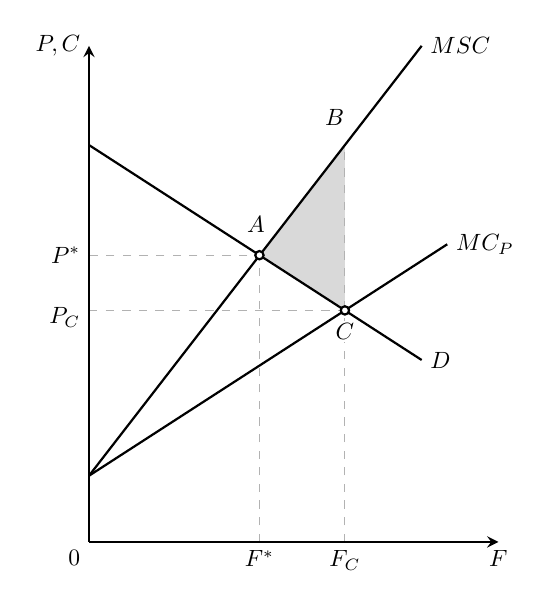
\begin{tikzpicture}[x=0.65cm, y=0.42cm, >=stealth, thick, every node/.style={scale=0.85}]
				% 1. 福利剩余区域填充 (最底层三角形 ABC)
				\fill[gray!30] (3.33, 8.67) -- (5, 12) -- (5, 7) -- cycle;
				
				% 2. 全局辅助虚线
				\draw[dashed, gray!60, thin] (3.33, 0) -- (3.33, 8.67) -- (0, 8.67);
				\draw[dashed, gray!60, thin] (5, 0) -- (5, 12);
				\draw[dashed, gray!60, thin] (0, 7) -- (5, 7);
				
				% 坐标轴标签物理分离防重叠微调
				\node[left] at (0, 8.67) {$P^*$};
				\node[left, yshift=-3pt] at (0, 7) {$P_C$};
				\node[below] at (3.33, 0) {$F^*$};
				\node[below] at (5, 0) {$F_C$};
				
				% 3. 坐标轴
				\draw[->] (0,0) -- (8,0) node[below] {$F$};
				\draw[->] (0,0) -- (0,15) node[left] {$P, C$};
				\node[below left] at (0,0) {$0$};
				
				% 4. 供需实线 (严格裁切定义域)
				\draw[domain=0:6.5, smooth, black] plot (\x, {2*\x + 2}) node[right] {$MSC$};
				\draw[domain=0:7.0, smooth, black] plot (\x, {\x + 2}) node[right] {$MC_P$};
				\draw[domain=0:6.5, smooth, black] plot (\x, {-\x + 12}) node[right] {$D$};
				
				% 5. 关键交点标号 (fill=white 消除交叉线干扰)
				\node[left, fill=white, inner sep=1pt] at (3.5, 9.6) {$A$};
				\node[above, fill=white, inner sep=1pt] at (4.8, 12.5) {$B$};
				\node[below, fill=white, inner sep=1pt] at (5, 6.7) {$C$};
				
				\fill[white] (3.33, 8.67) circle (1.5pt); \draw (3.33, 8.67) circle (1.5pt);
				\fill[white] (5, 7) circle (1.5pt); \draw (5, 7) circle (1.5pt);
			\end{tikzpicture}
		\end{center}
		
		\item \textbf{公共物品既是非竞争的，又是非排他的。解释这两个概念并清楚地说明它们之间的区别。}
		
		\textbf{答：} 非竞争性与非排他性是解构公共物品特性的两个完全独立的价格与技术维度。
		
		非竞争性聚焦于消费的边际成本维度，指在既定的生产品质下，向一个额外的新增消费者提供该商品的边际生产成本精确为零。
		这意味着一个人的享用行为并不会在物理或经济层面上剥蚀、减少任何其他人可获得的消费数量与质量。
		
		非排他性则聚焦于技术与产权控制维度，指在技术上完全无法阻止他人无偿享用该商品，或者实施排他性收费的法律行政管理成本高昂到在经济上完全不可行。
		
		两者的核心区别在于：非竞争性关注的是多一个人消费是否会增加全社会的生产成本，其核心是消费的无损性；而非排他性关注的是能否有效阻止未付费者偷越门槛，其核心是收费的不可行性。
		
		\item \textbf{一个村庄位于 1000 亩牧场附近。村庄拥有这片牧场，并且允许所有居民自由放牧，村庄的一些人暗示牧场过度放牧了。这可能是真的吗？这些人还建议村庄要么要求放牧者购买年度许可证，要么将牧场卖给放牧者。这些建议是否合适？}
		
		\textbf{答：} 该过度放牧的推断在微观经济学逻辑上完全成立。
		由于牧场属于公共财产，每个村民在决定增加羊群数量时，只会权衡个人的喂养收益与边际购买成本。
		他们绝不会主动考虑自己的放牧行为对草场植被造成的永久性破坏以及由此强加给全体村民的未来减产坏成本。
		这种私人成本与社会成本的系统性割裂，注定会引致草场的过度践踏与退化。
		
		村委会成员提出的两项政策建议均非常精准且切中时弊。
		课征年度许可证税本质上属于价格规制手段，它通过将许可证费用与放牧规模挂钩，强制将外部社会成本内生化为放牧者的私人边际成本。
		而将牧场直接确权并变卖给放牧者，则是通过科斯产权界定途径来化解危机。
		一旦公地转化为私人财产，所有者为了追求长期总财富的最大化，必然会主动限制当期的放牧头数，从而自发实现资源的跨期最优配置。
		\newpage
		\item \textbf{即使任何有电视机的人都能免费观看电视，公共电视还是有一部分是由私人捐款资助的。你能根据搭便车问题解释这一现象吗？}
		
		\textbf{答：} 公共电视具有极强的非排他性与非竞争性，是典型的纯公共物品。
		根据经典的理性经济人假设，在无法有效排他的公共消费环境下，人人都有强烈的动机隐藏真实偏好，拒绝为其付费，从而沦为搭便车者。
		这会导致纯粹的市场机制在供给公共物品时面临全面崩塌，最终的社会总供应量将远远低于社会最优水平。
		
		然而，现实中私人捐款的存在并不能颠覆搭便车理论，而是体现了消费者偏好的非均质性与非经济激励的补充。
		部分社会公众具有极高的边际消费收益，他们愿意独自承担发信成本以确保电视节目不中断，其捐款的私人收益已经能够覆盖边际成本。
		此外，社会成员并非完全孤立的理性计算机器，利他主义倾向、对社会责任感的自我认同以及特定企业的声誉广告效应，也会促使一部分人自发克服搭便车倾向，以自愿捐赠的次优形式维持公共物品的勉强运转。
		
		\item \textbf{在多数原则投票制决定公共支出水平时，解释为什么中间投票人结果不一定是有效率的。}
		
		\textbf{答：} 中间投票人定理表明，在单峰偏好及多数票决规则下，选举方案最终必将收敛于那位政治光谱处于最中间位置的选民所偏好的支出水平。
		然而，这一政治均衡在经济学意义上几乎总是缺乏效率的。
		帕累托有效的公共物品最优供给条件要求所有公民的边际意愿支付之和等于其边际提供成本。
		
		多数原则在统计偏好时，给每位公民的选票赋予了完全相同的绝对权重。
		它只粗暴地统计了赞成或反对的选民“数量”，却选择性忽略了不同选民背后的偏好“强度”。
		中间投票人可能对某项公共支出的边际感受极为温和，而少数激进或极度保守的选民可能对其抱有极为强烈的边际收益或损失。
		这种由于选票均等化导致的偏好强度错配，导致中间投票人的合意点无法在边际上达成全社会总剩余最大化的效率目标。
		
		\item \textbf{你认为维基百科是一种公共物品吗？它提供了正的外部性还是负的外部性？}
		
		\textbf{答：} 维基百科在本质上属于一种不完全的、具有准公共物品属性的网络数字资源。
		它展现出绝对的非竞争性，因为在互联网边际分发技术的支持下，新增一位用户在线检索词条所产生的边际服务器硬件成本微乎其微。
		然而，维基百科在技术与产权层面上并不具备绝对的非排他性。
		尽管其目前遵循免费开放的运营宗旨，但运营团队在法理上随时可以通过架设付费墙、限制注册或绑定身份等技术手段将不付费者完全阻断在外。
		
		在外部性维度上，维基百科呈现出极其明显的双向外溢效应。
		它主要释放了庞大的正外部性，通过无偿向全球公众沉淀高质量的信息库，大幅降低了全社会的知识获取门槛与搜寻成本，沉淀了宝贵的社会资本。
		但与此同时，它也带来了不可忽视的边际负外部性。
		海量且廉价的现成文本在客观上大幅降低了部分学生在撰写学术论文时的剽窃与洗稿成本，这反而迫使整个教育系统必须支付更高昂的软件检测与师资核查成本。
	\end{enumerate}
	\newpage
	\section{练习题}
	\begin{enumerate}[label=\textbf{\arabic*.}, leftmargin=*]
		\item \textbf{在居民住宅占去了一个城镇的东部后，有几家厂商定位在西部。每家厂商生产相同的产品，并在生产中排放有害气体，对社区的居民产生不利的影响。
			（1）为什么存在厂商产生的外部性？
			（2）你认为私下的谈判能够解决这一外部性问题吗？请解释。
			（3）社区可能会怎样决定空气质量的有效水平？}
		
		\textbf{答：} （1）厂商在生产过程中将有害气体直接排入大气，给东部居民的身体健康和生活质量带来了实质性损害。
		由于缺乏环境产权约束，厂商无需为这种向外施加的健康损害支付任何经济补偿。
		这导致厂商的私人生产成本显著低于真实的社会总成本，在市场上表现为生产领域的负外部性。
		
		（2）在实际运行中，私下谈判几乎无法有效化解该项外部不经济。
		一方面，该城镇的清洁空气产权并未在法律层面上明确界定给居民或厂商，谈判缺乏合法的博弈起点。
		另一方面，西部厂商与东部众多居民之间面临着极高的人员协调、信息搜寻与契约谈判等交易费用。
		居民内部还会滋生理性的免费搭便车动机，导致集体行动流产，无法达成帕累托改善。
		
		（3）社区应当通过加总所有受害家庭为了改善空气质量而愿意支付的边际意愿金额，构建出总边际收益曲线。
		随后，监管部门需将该总边际收益与厂商削减污染的边际治理成本进行横向联立。
		当全社区的总边际收益在交点处精确等于边际减污成本时，即可锁定全社会最优的空气质量与排污水平。
		
		\item \textbf{一个电脑编程人员游说反对对软件进行版权保护。他的论点是，每个人都应当从为个人电脑编写的创新程序中获益，与各种各样电脑程序的接触甚至会鼓舞年轻的编程人员编出更多的创新程序。考虑到由于他的建议而可能得到的边际社会收益，你同意该编程人员的主张吗？}
		
		\textbf{答：} 坚决反对该编程人员的主张，这一看似能够扩大社会收益的建议在激励机制上是短视且不可行的。
		软件研发具有高昂的前期沉淀成本以及近乎为零的边际复制成本，带有极强的正外部性与非排他性。
		一旦彻底取消版权保护，软件将沦为事实上的公共物品，任何效用享有者都可以通过免费搭便车来无偿攫取创新成果。
		
		这种制度安排会彻底剥夺开发者回收研发成本并获取边际风险回报的法律资格。
		理性的软件厂商在面对私人边际收益归零的困境时，将选择大幅削减研发投入甚至完全退出创意市场。
		虽然短期内由于零价格复制使得边际社会收益看似扩大，但长期来看将导致创新的彻底枯竭，造成不可挽回的社会总福利福利损失。
		
		\item \textbf{假定科学研究提供了关于二氧化硫排放的收益和成本的一些信息：减少排放量的收益：$MB = 500 - 20A$；减少排放量的成本：$MC = 200 + 5A$。其中 A 表示减少的排放的数量，单位是百万吨。收益和成本的单位是美元/吨。
			（1）社会的最优减污量是多少？
			（2）在社会最优处，减污的边际收益和边际成本是多少？
			（3）如果减污量超过社会最优水平 100 万吨，社会净收益怎么变化？减少 100 万吨呢？
			（4）为什么当边际收益等于边际成本而不是总收益等于总成本时达到社会最优？}
		
		\textbf{答：} （1）为了最大化环境治理的社会净收益，必须满足边际收益等于边际成本的一阶最优化条件：
		\[
		500 - 20A = 200 + 5A \implies 25A = 300 \implies A = 12 \text{（百万吨）}
		\]
		因此，社会最优的二氧化硫减排量为 12 百万吨。
		
		（2）将最优减排量 $A = 12$ 分别代入收益与成本函数中，可以求得最优处的边际指标：
		\[
		\begin{aligned}
			MB &= 500 - 20 \times 12 = 260 \text{（美元/吨）} \\
			MC &= 200 + 5 \times 12 = 260 \text{（美元/吨）}
		\end{aligned}
		\]
		即在社会最优均衡点处，减污的边际收益与边际成本完全相等，均为 260 美元/吨。
		
		（3）当减排量过度推进至 13 百万吨（超标 100 万吨）时，多减这一单元所承载的边际成本将跨越边际收益，在社会剩余中撕裂出无谓损失三角形 $E$：
		\[
		\Delta \pi = -0.5 \times (MC - MB) \times \Delta A = -0.5 \times (265 - 240) \times 1 = -12.5 \text{（百万美元）}
		\]
		同理，当减排量不足，锁死在 11 百万吨（少减 100 万吨）时，未能斩获的净收益表现为少减造成的无谓损失三角形 $D$：
		\[
		\Delta \pi = -0.5 \times (MB - MC) \times \Delta A = -0.5 \times (280 - 255) \times 1 = -12.5 \text{（百万美元）}
		\]
		由此可见，无论是过度减污还是减污不足，均会导致全社会总收益相比于最优状态萎缩 12.5 百百万美元。
		
		\begin{center}
			\small
			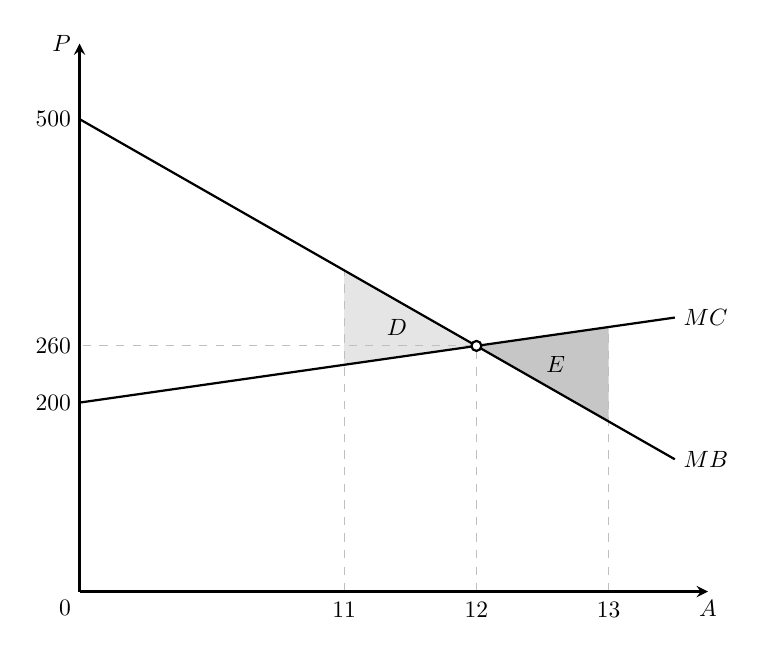
\begin{tikzpicture}[x=0.42cm, y=1.2cm, >=stealth, thick, every node/.style={scale=0.85}]
				% 1. 福利无谓损失区域填充 (处于最底层，利用非对称放大技术将阴影面积拓展至最佳视觉比例)
				\fill[gray!20] (8, 2.4) -- (12, 2.6) -- (8, 3.4) -- cycle;   % 减污不足引起的福利损失区 D
				\fill[gray!45] (12, 2.6) -- (16, 2.8) -- (16, 1.8) -- cycle; % 过度减污引起的福利损失区 E
				
				% 2. 全局辅助虚线 ( thin 减噪线宽)
				\draw[dashed, gray!50, thin] (12, 0) -- (12, 2.6) -- (0, 2.6);
				\draw[dashed, gray!50, thin] (8, 0) -- (8, 3.4);
				\draw[dashed, gray!50, thin] (16, 0) -- (16, 2.8);
				
				% 3. 坐标轴标签物理分离技术 (彻底避免文字与轴线交织重叠)
				\node[left] at (0, 2.6) {$260$};
				\node[left] at (0, 5) {$500$};
				\node[left] at (0, 2) {$200$};
				
				\node[below, yshift=-1pt] at (12, 0) {$12$};
				\node[below, yshift=-1pt] at (8, 0) {$11$};  % 物理坐标放大至 8 处，标签严格复刻 11
				\node[below, yshift=-1pt] at (16, 0) {$13$}; % 物理坐标放大至 16 处，标签严格复刻 13
				
				% 4. 坐标轴主干
				\draw[->] (0,0) -- (19,0) node[below] {$A$};
				\draw[->] (0,0) -- (0,5.8) node[left] {$P$};
				\node[below left] at (0,0) {$0$};
				
				% 5. 供需实线 (严格根据排版版心裁切定义域 domain)
				\draw[domain=0:18, smooth, black] plot (\x, {5 - 0.2*\x}) node[right] {$MB$};
				\draw[domain=0:18, smooth, black] plot (\x, {2 + 0.05*\x}) node[right] {$MC$};
				
				% 6. 核心区域与均衡点打靶 (fill=white 擦除背景线段，保证极致可读性)
				\node[black] at (9.6, 2.8) {$D$};
				\node[black] at (14.4, 2.4) {$E$};
				\fill[white] (12,2.6) circle (1.8pt); \draw (12,2.6) circle (1.8pt);
			\end{tikzpicture}
		\end{center}
		
		（4）资源配置最优的核心逻辑是追求社会总剩余（总收益与总成本之差）的极大化，而非两者的数值对等。
		根据微观数学优化原理，极大化总剩余的充要条件是其一阶导数归零，即最后一单位减污带来的边际社会收益必须恰好冲平其边际社会成本。
		若错误地将目标锚定在总收益等于总成本的交点上，意味着将社会净收益榨取至零，从而导致了减排过度，引发了严重的社会资源低效率浪费。
		
		\item \textbf{处于不同地点的四家厂商向一条河中倾倒不同数量的废水。废水对住在下游的房屋主人的游泳质量产生不利影响。这些人可以建造游泳池来避免到河中游泳，而厂商可以购买过滤设备，消除向河中倾倒的物质中的有害化学成分。作为一个地区计划组织的政策顾问，你将如何比较和对照下列对付废水有害影响的选择：
			（1）对位于河边的厂商收同样费率的废水排放费。
			（2）对每家厂商可以倾倒的废水水平规定同样的标准。
			（3）实行可转让废水许可证制度，它确定废水的总水平并给所有的厂商一样的许可证。}
		
		\textbf{答：} （1）实施统一样例的废水排放费属于价格型经济规制。
		该费用的推行要求规制机构必须精准掌握下游居民的边际受损收益函数和各家厂商的边际治理成本。
		在开征后，各厂商将自发削减排污，直至其个体减污的边际成本与法定的排放费率在边际上完全相等。
		当四家厂商面对异质性的减污技术时，排放费能够自发诱导低成本厂商多减污、高成本厂商少减污，从而以最低的总社会成本达成污染控制目标。
		
		（2）规定同样的排污标准属于典型的一刀切式数量管制手段。
		当四家厂商的减污技术存在显著代数差异，即边际减污成本曲线不重合时，强行施加均等的实物标准将剥夺低成本企业的治理优势。
		这不仅无法达成社会总减污成本的最小化，还会由于缺乏多减排的超额利润激励，导致各厂商完全失去引入升级版过滤设备的研发动力。
		
		（3）可转让废水许可证制度则是将标准的总量锁定优势与排污费的成本分配效率完美兼顾的集大成机制。
		地区组织只需率先核定该河流生态所能承受的废水总容量，并在初期将许可证均等分发给四家厂商。
		许可证在二级市场的自由买卖将迅速催生出有效的权利均衡价格。
		低治理成本的厂商会通过加速过滤并出让盈余许可证来变现，高成本厂商则会通过买入许可证来对冲惩罚。
		该机制既确保了环境总质量绝对不超标，又成功利用市场看不见的手将减污负担自发配置给效率最高的企业。
		
		\item \textbf{在医学研究表明二手烟对健康有负外部效应后，最近的社会倾向表示出对在公共场合吸烟越来越不能忍受。许多人指出了二手烟对健康的负效应。如果你是一个吸烟者，并且你希望继续吸烟，而不管反吸烟法规有多严厉，描述下列立法建议对你行为的影响。从这些计划的结果看，你作为一个吸烟者是否受益？社会作为一个整体是否受益？
			（1）一项提议法案要求降低所有香烟中的焦油和尼古丁。
			（2）对每包香烟征税。
			（3）对出售的每包香烟征税。
			（4）要求吸烟者在所有时候都携带吸烟许可证，这些许可证由政府出售。}
		
		\textbf{答：} 公共场合吸烟属于典型的消费负外部性。上述立法旨在将外部受损成本内生化，吸烟者作为污染制造者，在任何方案下均不会获得个人经济利益的改善。社会整体福利是否增加，则取决于外部性削减收益与行政实施成本的边际权衡。
		
		（1）该法案相当于设定了排污的技术标准。由于上瘾依赖性，吸烟者为了维持每日摄入的焦油和尼古丁总量，必然会选择大幅增加吸烟频率与数量。这导致吸烟者的总支出上升，而公共环境中的二手烟总量并未实质性下降，社会总福利可能不增反减。
		
		（2）与（3）无论是向买方征税还是向卖方征税，最终的税收转嫁与经济归宿完全等价。征税大幅拉升了香烟的含税均衡价格，其对吸烟者行为的抑制程度取决于香烟的需求价格弹性。若弹性较低，社会将主要获得财政税收，而环境改善较为有限。
		
		（4）该许可证机制等价于可转让排污权模式。由于许可证由政府统筹出售，这实际上是将环境产权明确界定给非吸烟群体，实现了福利由吸烟者向全社会的逆向转移。其面临的核心障碍是政府高昂的常态化稽查与准入管理成本。
		
		\item \textbf{美国某一地区纸品市场的需求曲线和供给曲线如下：$Q_D = 160000 - 2000P$，$Q_S = 40000 + 2000P$。$Q_D$ 是需求数量，$Q_S$ 是供给数量，单位是百磅，P 表示每百磅的价格。目前尚没有任何管制造纸厂向河中排放废水的措施，结果造成了大量的废水排放。生产纸的边际外部成本（MEC）由曲线 $MEC = 0.0006Q_S$ 给出。
			（1）计算在没有任何规制措施下，竞争性产出和价格是多少？
			（2）计算最优社会产量和价格。
			（3）解释为什么（1）和（2）的答案不同。}
		
		\textbf{答：} （1）在自由放任的市场环境下，均衡条件由供求曲线交点决定，即满足 $Q_D = Q_S$：
		\[
		160000 - 2000P = 40000 + 2000P \implies 40000P = 120000
		\]
		解得竞争性均衡价格为 $P = 30$ 美元/百磅，代入求得完全竞争产出为 $Q = 100000$ 百磅。
		
		（2）首先由供给曲线反推反供给函数，该函数在经济学上等价于厂商的私人边际成本：
		\[
		P = 0.0005Q_S - 20 \implies MC = 0.0005Q
		\]
		将边际外部成本融入私人成本中，从而推导出真实的边际社会成本函数：
		\[
		MSC = MC + MEC = 0.0005Q - 20 + 0.0006Q = 0.0011Q - 20
		\]
		由反需求函数获得边际社会收益函数 $MSB = 80 - 0.0005Q$。令 $MSC = MSB$ 实现社会最优：
		\[
		0.0011Q - 20 = 80 - 0.0005Q \implies 0.0016Q = 100 \implies Q^* = 62500 \text{（百磅）}
		\]
		将最优数量代入反需求函数，求得最优社会价格为 $P^* = 80 - 0.0005 \times 62500 = 48.75$ 美元/百磅。
		
		（3）计算结果的差异根源于市场主体决策时对外部成本的视而不见。
		自由竞争下厂商仅依据私人边际成本定价，造成了严重的产量过剩与价格低估。
		社会最优路径强制要求企业为排放废水的外溢损害承担责任，导致供给曲线上移并推高了最终价格。
		
		\begin{center}
			\small
			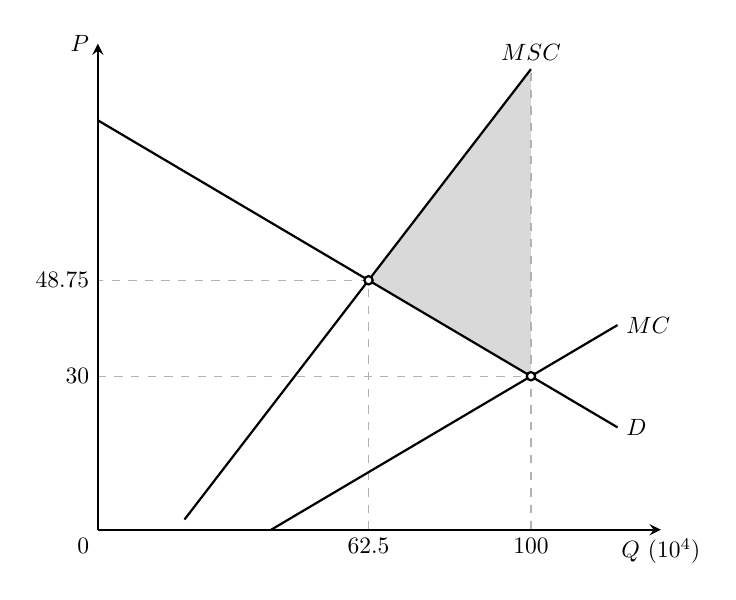
\begin{tikzpicture}[x=0.55cm, y=0.65cm, >=stealth, thick, every node/.style={scale=0.85}]
				% 1. 损失阴影区域
				\fill[gray!30] (6.25, 4.875) -- (10, 3) -- (10, 9) -- cycle;
				
				% 2. 辅助虚线
				\draw[dashed, gray!60, thin] (6.25, 0) -- (6.25, 4.875) -- (0, 4.875);
				\draw[dashed, gray!60, thin] (10, 0) -- (10, 9);
				\draw[dashed, gray!60, thin] (0, 3) -- (10, 3);
				
				% 标签物理分离微调
				\node[left] at (0, 3) {$30$};
				\node[left] at (0, 4.875) {$48.75$};
				\node[below] at (6.25, 0) {$62.5$};
				\node[below] at (10, 0) {$100$};
				
				% 3. 坐标轴 (数量以万磅为单位映射)
				\draw[->] (0,0) -- (13,0) node[below] {$Q\ (10^4)$};
				\draw[->] (0,0) -- (0,9.5) node[left] {$P$};
				\node[below left] at (0,0) {$0$};
				
				% 4. 供需实线
				\draw[domain=4:12, smooth, black] plot (\x, {0.5*\x - 2}) node[right] {$MC$};
				\draw[domain=2:10, smooth, black] plot (\x, {1.1*\x - 2}) node[above] {$MSC$};
				\draw[domain=0:12, smooth, black] plot (\x, {8 - 0.5*\x}) node[right] {$D$};
				
				% 5. 交点标号
				\fill[white] (10,3) circle (1.5pt); \draw (10,3) circle (1.5pt);
				\fill[white] (6.25,4.875) circle (1.5pt); \draw (6.25,4.875) circle (1.5pt);
			\end{tikzpicture}
		\end{center}
		
		\item \textbf{在干洗市场中，逆市场需求曲线为 P=100-Q，总体(私人)边际社会成本 $MC=10+Q$ 。最后，干洗过程产生的污染导致的边际外部成本 MEC=Q。
			（1）计算在没有规制的情况下，竞争性产出和价格。
			（2）计算社会最优产出和价格。
			（3）计算使得市场竞争产量等于社会最优产量的税收水平。
			（4）计算在没有管制时，垄断厂商的产出和价格。
			（5）计算使得垄断厂商的产量等于社会最优产量的税收水平。
			（6）若没有规制的打算，哪一种市场结构的社会福利更高？试讨论。}
		
		\textbf{答：} （1）完全竞争厂商在无视污染时满足价格等于私人边际成本条件，即 $100 - Q = 10 + Q$。解得自发市场竞争产出为 $Q_c = 45$，对应的均衡价格为 $P_c = 55$。
		
		（2）将环境污染并入考量，推导出全社会的边际总成本函数为：
		\[
		MSC = MC + MEC = 10 + Q + Q = 10 + 2Q
		\]
		令边际社会总成本等于反需求收益函数：$10 + 2Q = 100 - Q \implies 3Q = 90$。解得社会最优产出为 $Q^* = 30$，对应的社会合意最优价格为 $P^* = 70$。
		
		（3）政府应课征特定从量税 $t$，使厂商感受到的调整后边际成本移至 $MC' = MC + t = 10 + Q + t$。为强行引导竞争性产量收敛至最优规模 $Q^* = 30$，需满足：
		\[
		P(30) = MC'(30) \implies 70 = 10 + 30 + t \implies t = 30
		\]
		此时的税收水平应精准等于最优产出处的边际外部损害成本，即 $t = MEC(30) = 30$。
		
		（4）垄断厂商在无规制时，面临的边际收益函数为 $MR = 100 - 2Q$。依据利润最大化准则 $MR = MC$ 进行独立决策：
		\[
		100 - 2Q = 10 + Q \implies 3Q = 90
		\]
		求得无管制的垄断均衡产出为 $Q_m = 30$，带入需求曲线得到垄断市场价格为 $P_m = 70$。
		
		（5）由于无管制的垄断厂商出于攫取垄断利润的目的而天然具有限产动机，其自发吐出的产量（30）在数值上恰好与社会最优资源配置量完全吻合，因此无需施加任何额外的宏观税收手段，即最优税收水平 $t = 0$。
		
		（6）在缺乏宏观环境规制的前设下，垄断市场结构的社会总福利显著高于完全竞争市场。
		完全竞争机制由于对负外部性的完全放任，引发了灾难性的过度生产，制造了大量的环境污染。
		而垄断势力所引致的“产出不足”扭曲，在代数方向上刚好对冲了负外部性导致的“过度产出”扭件。
		两个原本各自引发失灵的负向机制在边际上完美交织、相互抵消，使得垄断行业的最终社会剩余反而锁定了帕累托最优状态。
		
		\item \textbf{回忆例 18.5 中的全球变暖问题，教材表 18-3 显示了每年减少 1\% 温室气体排放所带来的净收益，什么样的折现率能够刚好使得 NPV 等于 0?}
		
		\textbf{答：} 教材所给的分段表格仅显示了每十年的跨期净收益，由于年度间的福利效应非线性变动，无法直接用于精准计算项目的净现值。
		为了精确锁定使净现值（NPV）归零的临界折现率，必须构建包含 101 年逐年连续观测值的精算矩阵。
		通过将初始年份 2010 年定义为基准时间点 0，并让时间变量逐年递增，可以对各期现金流进行精准贴现。
		
		当折现率设定为 1.3\% 时，全期贴现后的净收益现值总额（NPV）为 21.3 美元。
		利用数值试错法不断调整贴现率以逼近零位交点，可以测算出当折现率精准达到 2.09\% 时，前期的环境治理成本与远期的跨周期环境红利现值将完全冲平。
		在缺乏连续微观数据时，若采用线性插值法补齐缺失年份，推导出的临界折现率约为 2.14\%。
		若采用几何拟合方式，将不同折现率下的净现值绘制成平滑曲线，其与零位横轴的交点同样稳健地指向 2.1\% 的政策平衡点。
		
		\begin{center}
			\footnotesize
			\renewcommand{\arraystretch}{1.2}
			\begin{tabular*}{\linewidth}{@{\extracolsep{\fill}}cccccccc}
				\hline
				年份 & 净收益 & 年份 & 净收益 & 年份 & 净收益 & 年份 & 净收益 \\ \hline
				2010 & -0.650 & 2035 & -0.813 & 2060 & -1.266 & 2085 & 2.139  \\
				2011 & -0.658 & 2036 & -0.818 & 2062 & -1.199 & 2086 & 2.377  \\
				2012 & -0.665 & 2037 & -0.822 & 2062 & -1.127 & 2087 & 2.625  \\
				2013 & -0.673 & 2038 & -0.825 & 2063 & -1.051 & 2088 & 2.884  \\
				2014 & -0.680 & 2039 & -0.829 & 2064 & -0.970 & 2089 & 3.154  \\
				2015 & -0.688 & 2040 & -0.832 & 2065 & -0.885 & 2090 & 3.436  \\
				2016 & -0.695 & 2041 & -0.834 & 2066 & -0.795 & 2091 & 3.730  \\
				2017 & -0.702 & 2042 & -0.837 & 2067 & -0.700 & 2092 & 4.036  \\
				2018 & -0.710 & 2043 & -0.838 & 2068 & -0.599 & 2093 & 4.356  \\
				2019 & -0.717 & 2044 & -0.840 & 2069 & -0.493 & 2094 & 4.689  \\
				2020 & -0.724 & 2045 & -0.841 & 2070 & -0.382 & 2095 & 5.036  \\
				2021 & -0.731 & 2046 & -0.841 & 2071 & -0.264 & 2096 & 5.397  \\
				2022 & -0.738 & 2047 & -0.841 & 2072 & -0.141 & 2097 & 5.774  \\
				2023 & -0.745 & 2048 & -0.874 & 2073 & -0.011 & 2098 & 6.165  \\
				2024 & -0.751 & 2049 & -0.839 & 2074 & 0.126  & 2099 & 6.573  \\
				2025 & -0.758 & 2050 & -0.838 & 2075 & 0.269  & 2100 & 6.997  \\ \hline
				2026 & -0.764 & 2051 & -0.912 & 2077 & 0.578  & 2102 & 7.898  \\
				2027 & -0.770 & 2052 & -0.951 & 2078 & 0.743  & 2103 & 8.375  \\
				2028 & -0.777 & 2053 & -0.951 & 2078 & 0.743  & 2103 & 8.375  \\
				2029 & -0.782 & 2054 & -0.992 & 2079 & 0.916  & 2104 & 8.871  \\
				2030 & -0.788 & 2055 & -1.033 & 2080 & 1.098  & 2105 & 9.387  \\
				2031 & -0.794 & 2054 & -1.077 & 2081 & 1.288  & 2106 & 9.923  \\
				2032 & -0.799 & 2057 & -1.122 & 2082 & 1.487  & 2107 & 10.480 \\
				2033 & -0.804 & 2058 & -1.168 & 2083 & 1.695  & 2108 & 11.059 \\
				2034 & -0.809 & 2059 & -1.216 & 2084 & 1.912  & 2109 & 11.660 \\
				&        &      &        &      &        & 2110 & 12.284 \\ \hline
			\end{tabular*}
		\end{center}
		\newpage
		\item \textbf{一个养蜂人住在一个苹果园旁边。果园主人由于蜜蜂而受益，因为每箱蜜蜂大约能为一英亩果树授粉。然而，果园主人并不为这一服务支付任何钱，因为蜜蜂并不需要他做任何事就会到果园来。蜜蜂并不足以使全部果园都授到粉，因此果园主人必须以每英亩果树 10 美元的成本，用人工来完成授粉。养蜂人的边际成本为 $MC = 10 + 5Q$，式中，Q 是蜂箱数目。每箱产生价值 40 美元的蜂蜜。
			（1）养蜂人将会持有多少箱蜜蜂?
			（2）这是不是经济上有效率的蜂箱数目?
			（3）什么样的变动可以导致更有效率的运作？}
		
		\textbf{答：} （1）在缺乏外部协调的放任市场中，自利的养蜂人仅根据私人边际收益等于边际成本的准则来决定蜂箱供给。
		蜂蜜的市场价值构成其唯一的边际收益流，其最优决策方程为：
		\[
		40 = 10 + 5Q \implies 5Q = 30 \implies Q = 6 \text{（箱）}
		\]
		因此，在无规制状态下，养蜂人自发持有的蜂箱规模为 6 箱。
		
		（2）这一自发均衡在全社会视角下是完全缺乏经济效率的。
		养蜂活动为相邻的果树提供了免费的生态传粉服务，强加给市场一个显著的正外部性。
		果园主人因蜜蜂授粉而免除了每英亩 10 美元的人工授粉开支，这意味着每增加一箱蜜蜂，全社会获得的边际外部收益为 10 美元。
		包含外部溢价的边际社会收益应当升至 50 美元，私人决策严重低估了生态价值，导致了生产不足。
		若果园主人愿意将节省下的人工授粉款项补贴给养蜂人，其边际激励方程将跃升为：
		\[
		40 + 10 = 10 + 5Q \implies 5Q = 40 \implies Q = 8 \text{（箱）}
		\]
		精算表明，全社会合意的高效蜂箱规模应当是 8 箱。
		
		（3）引导产权纵向一体化合并是彻底化解该项配置扭曲的内在途径。
		通过将果园与养蜂场合并为单一的生态农业企业，原本外溢的授粉红利将直接在企业内部实现闭环。
		在维持独立主体的格局下，双方也可通过自愿签署附带约束的互惠契约，由果园主向养蜂人按蜂箱数量支付特定生态津贴，从而自发驱使微观产量收敛至全社会最优规模。
		
		\item \textbf{在一个社区内有三个集团。它们对公共电视节目小时数 T 的需求曲线分别是：$W_1 = 200 - T$，$W_2 = 240 - 2T$，$W_3 = 320 - 2T$。假定公共电视是一种纯粹的公共产品，它能以每小时 200 美元的不变边际成本生产出来。
			（1）公共电视有效率的小时数是多少？
			（2）一个竞争性的私人市场会提供多少公共电视？}
		
		\textbf{答：} （1）由于纯公共物品在消费上表现出绝对的非竞争性，全社会对电视节目的总边际收益应当在给定的数量点上进行垂直加总。
		当播放时长满足 $100 < T \le 112$ 时，三大集团的边际意愿支付均大于零，此时通过重叠加总构建出社会总边际收益（MSB）函数：
		\[
		MSB = (200 - T) + (240 - 2T) + (320 - 2T) = 760 - 5T
		\]
		令社会总边际收益在边际上精确等于其不变提供成本：
		\[
		760 - 5T = 200 \implies 5T = 560 \implies T^* = 112 \text{（小时）}
		\]
		计算表明，全社会整体最优的公共电视播放小时数应为 112 小时。
		
		\begin{center}
			\small
			\renewcommand{\arraystretch}{1.2}
			\setlength{\tabcolsep}{6pt}
			\begin{tabular}{ccccc}
				\hline
				小时数 & 集团 1 & 集团 2 & 集团 3 & 垂直加总 (MSB) \\ \hline
				100    & 100    & 40     & 120    & 260            \\
				106    & 94     & 28     & 108    & 230            \\
				112    & 88     & 16     & 96     & 200            \\
				118    & 82     & 4      & 84     & 170            \\ \hline
			\end{tabular}
		\end{center}
		
		（2）若诉诸完全竞争的私人市场，非排他性带来的搭便车顽疾将导致垂直加总溢价完全解体。
		私人资本无法向未付费者实施价格排他，其供给决策只能退化为盯住单一主体的独立私人边际收益。
		当市场均衡价格在竞争压力下等同于边际成本 200 美元时，各集团根据自身意愿独立核定购买数量：
		集团 1 的最高边际估价恰为 200，在市价 200 下的需求量为 0；
		集团 2 满足 $240 - 2T = 200$，求得独立需求为 20 小时；
		集团 3 满足 $320 - 2T = 200$，求得独立需求为 60 小时。
		私人市场通过横向加总各主体的排他性需求，最终仅能挤出 80 小时的服务，公共福利缩减严重。
		
		\item \textbf{重新考虑教材中例 18.7 中的共有资源问题。假设龙虾的受欢迎程度继续提高，需求曲线从 $C = 0.401 - 0.0064F$ 变为 $C = 0.50 - 0.0064F$ 。这一需求的转变会如何影响龙虾的实际捕捉量和有效率的捕捉量，以及共同进入的社会成本？（提示：利用例子中给出的边际社会成本曲线和边际私人成本曲线。）}
		
		\textbf{答：}
		由于消费者对龙虾的偏好提高，龙虾的市场需求曲线向右上平移。
		
		社会有效率的捕捉量 $F^*$ 由新需求曲线与边际社会成本曲线的交点决定。联立两方程：
		\[
		0.50 - 0.0064F = -5.645 + 0.6509F
		\]
		解得有效捕捉量 $F^* \approx 9.35$ 百万磅。
		
		在自由准入的共有产权状态下，捕捞者会持续进入直到经济利润为零。此时，需求曲线与边际私人成本曲线相交：
		\[
		0.50 - 0.0064F = -0.357 + 0.0573F
		\]
		解得市场实际捕捉量 $F_c \approx 13.45$ 百万磅。
		
		计算结果表明，需求的上升使得有效捕捉量和实际捕捉量均有所增加。但由于缺乏产权保护，实际捕捉量远高于社会有效水平。
		
		当实际捕捉量达到 $13.45$ 百万磅时，消费者的边际估价降至 $0.41$，而真实的边际社会成本则高达 $3.11$。
		
		这在过度捕捞区间 $[9.35, 13.45]$ 内造成了无谓损失，即下图中由 $A, B, C$ 三点构成的阴影三角形。共同进入的社会成本为：
		\[
		\text{社会成本} = \frac{1}{2} \times (13.45 - 9.35) \times (3.11 - 0.41) = 5.535 \text{（百万美元）}
		\]
		与需求改变前相比，市场需求的扩张加剧了共有资源产权缺失带来的无效率，导致共同进入的社会福利代价显著上升。
		
		\begin{center}
			\small
			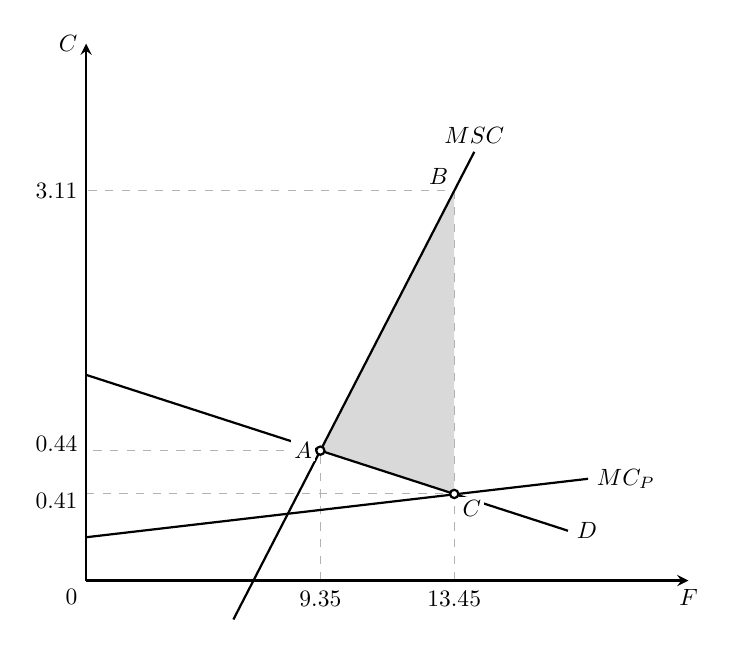
\begin{tikzpicture}[x=0.85cm, y=1.1cm, >=stealth, thick, every node/.style={scale=0.85}]
				% 1. 福利剩余区域填充 (处于最底层，采用轻量学术灰)
				\fill[gray!30] (3.5, 1.5) -- (5.5, 4.5) -- (5.5, 1.0) -- cycle;
				
				% 2. 全局辅助虚线 (thin 减噪线宽)
				\draw[dashed, gray!60, thin] (3.5, 0) -- (3.5, 1.5) -- (0, 1.5);
				\draw[dashed, gray!60, thin] (5.5, 0) -- (5.5, 4.5) -- (0, 4.5);
				\draw[dashed, gray!60, thin] (0, 1.0) -- (5.5, 1.0);
				
				% 坐标轴标签物理分离防重叠微调
				\node[left] at (0, 4.5) {$3.11$};
				\node[left, yshift=3pt] at (0, 1.5) {$0.44$};
				\node[left, yshift=-3pt] at (0, 1.0) {$0.41$};
				\node[below, yshift=-1pt] at (3.5, 0) {$9.35$};
				\node[below, yshift=-1pt] at (5.5, 0) {$13.45$};
				
				% 3. 坐标轴 (适度外延纵轴与横轴，为标签腾出呼吸空间)
				\draw[->] (0,0) -- (9.0,0) node[below] {$F$};
				\draw[->] (0,0) -- (0,6.2) node[left] {$C$};
				\node[below left] at (0,0) {$0$};
				
				% 4. 供需实线 (精细裁切 MSC 定义域至 5.8，彻底解决溢出)
				\draw[domain=2.2:5.8, smooth, black] plot (\x, {1.5*\x - 3.75}) node[above] {$MSC$};
				\draw[domain=0:7.5, smooth, black] plot (\x, {0.09*\x + 0.5}) node[right] {$MC_P$};
				\draw[domain=0:7.2, smooth, black] plot (\x, {-0.25*\x + 2.375}) node[right] {$D$};
				
				% 5. 核心交点标号 (fill=white 强力擦除背景交叉线段干扰)
				\node[left, fill=white, inner sep=1.2pt, xshift=-2pt] at (3.5, 1.5) {$A$};
				\node[above left, fill=white, inner sep=1.2pt, xshift=-1pt, yshift=1pt] at (5.5, 4.5) {$B$};
				\node[below right, fill=white, inner sep=1.2pt, xshift=2pt, yshift=-1pt] at (5.5, 1.0) {$C$};
				
				\fill[white] (3.5, 1.5) circle (1.5pt); \draw (3.5, 1.5) circle (1.5pt);
				\fill[white] (5.5, 1.0) circle (1.5pt); \draw (5.5, 1.0) circle (1.5pt);
			\end{tikzpicture}
		\end{center}
		
		\item \textbf{乔治海滩是新英格兰海岸外鱼的高产地区，但根据鱼的总数可分为两个区域。1 区每平方英里鱼的总数较高，但它对捕鱼努力来说是报酬严重递减的。1 区每天的捕捞量（以吨计算）是：$F_1 = 200X_1 - 2(X_1)^2$。式中，$X_1$ 是在那里捕鱼的船只数目。2 区每平方英里的鱼少些，但也大些，并且报酬递减也不那么成问题。它每天的捕捞量是：$F_2 = 100X_2 - (X_2)^2$。式中，$X_2$ 是在 2 区捕鱼的船只数目。各区的边际捕捞量由下式给出：$MFC_1 = 200 - 4X_1$，$MFC_2 = 100 - 2X_2$。现在有 100 条船得到美国政府许可在这两个区域捕鱼。鱼以每吨 100 美元出售。每条船的总成本（资本和运作）为每天不变的 1000 美元。就这一情况回答下列问题：}\\
		\textbf{（1）如果船都能在他们想去的地方捕鱼，政府不加限制，每个区域将有多少条船捕鱼？捕捞的总值将是多少？}\\
		\textbf{（2）如果美国政府能够限制船只，每个区域应当配置多少条船？捕捞的总值将是多少？假定船的总数仍为 100。}\\
		\textbf{（3）如果另有渔民想购买船只，加入捕鱼队伍，一个希望捕鱼净值最大化的政府是否应当给他们许可证，让他们捕鱼？为什么？}
		
		\textbf{答：}
		（1）在无限制的自由准入状态下，船只可以在两个区域自由选择。如果某个区域的平均捕捞量较高，就会吸引更多船只前往，直到两个区域的平均捕捞量相等。
		
		根据题意，两区域各自的平均捕捞量方程为：
		\[
		\begin{aligned}
			AF_1 &= \frac{F_1}{X_1} = 200 - 2X_1 \\
			AF_2 &= \frac{F_2}{X_2} = 100 - X_2
		\end{aligned}
		\]
		
		结合 100 条船的总量限制条件 $X_1 + X_2 = 100$，令两区域的平均捕捞量相等：
		\[
		200 - 2X_1 = 100 - (100 - X_1) \implies 3X_1 = 200
		\]
		解得 1 区的船只数量 $X_1 \approx 66.67$ 条，2 区的船只数量 $X_2 \approx 33.33$ 条。
		
		将各区的船只数量带回原捕捞量函数，可以计算出两个区域的实际日捕捞量：
		\[
		\begin{aligned}
			F_1 &= 200 \times \left(\frac{200}{3}\right) - 2 \times \left(\frac{200}{3}\right)^2 \approx 4444.44 \text{（吨）} \\
			F_2 &= 100 \times \left(\frac{100}{3}\right) - \left(\frac{100}{3}\right)^2 \approx 2222.22 \text{（吨）}
		\end{aligned}
		\]
		全海域的总捕捞量为 $F = F_1 + F_2 \approx 6666.67$ 吨。在价格为每吨 100 美元时，总捕捞产值为 $6666.67 \times 100 = 666667$ 美元。
		
		（2）如果政府限制船只以使总捕捞量最大，应当重新分配船只，使得两个区域的边际捕捞量相等。
		
		联立两区域的边际捕捞量方程与船只总量约束：
		\[
		200 - 4X_1 = 100 - 2(100 - X_1) \implies 6X_1 = 300
		\]
		解得此时 1 区应当配置 $X_1 = 50$ 条船，2 区配置 $X_2 = 50$ 条船。
		
		将最优船只数量代入总捕捞量函数，得到调整后的各区捕捞量：
		\[
		\begin{aligned}
			F_1 &= 200 \times 50 - 2 \times 50^2 = 5000 \text{（吨）} \\
			F_2 &= 100 \times 50 - 50^2 = 2500 \text{（吨）}
		\end{aligned}
		\]
		此时全海域的总捕捞量提高到 $F = 5000 + 2500 = 7500$ 吨。在价格为每吨 100 美元时，限制船只分配后的总捕捞产值为 $7500 \times 100 = 750000$ 美元。
		
		（3）政府不应当给他们发放新的许可证。要使整个捕鱼行业的净价值达到最大，应当让每个区域的边际捕捞产值等于单条船的每天运营成本（1000 美元）。
		
		由于鱼的价格为每吨 100 美元，我们可以分别求解两个区域在经济学效率最高时的最优船只规模：
		\[
		\begin{aligned}
			100 \times (200 - 4X_1) = 1000 &\implies X_1^* = 47.5 \text{（条）} \\
			100 \times (100 - 2X_2) = 1000 &\implies X_2^* = 45.0 \text{（条）}
		\end{aligned}
		\]
		
		计算表明，全海域最合适的总船数应当是 $47.5 + 45 = 92.5$ 条。
		
		目前市场上已经获准捕鱼的 100 条船已经超过了这一最佳规模。因此，政府不仅不应该发放新的许可证，反而应该通过合理手段减少现有的船只数量。
		\begin{center}
			\small
			\begin{tikzpicture}[x=0.55cm, y=0.42cm, >=stealth, thick, every node/.style={scale=0.9}]
				% ==================== LEFT GRAPH: ZONE 1 ====================
				\begin{scope}
					% 坐标轴
					\draw[->] (0,0) -- (8.5,0) node[below] {$X_1$};
					\draw[->] (0,0) -- (0,12) node[left] {$P$};
					\node[below left] at (0,0) {$0$};
					\node[above, font=\footnotesize\bfseries, yshift=2pt] at (4,12) {1区 (高密度递减区)};
					
					% 辅助虚线
					\draw[dashed, gray!50, thin] (5,0) -- (5,5);
					\draw[dashed, gray!50, thin] (6.67,0) -- (6.67,3.33) -- (0,3.33);
					
					% 标签微调防止重叠
					\node[below, yshift=-1pt] at (5,0) {\scriptsize 50};
					\node[below, xshift=4pt, yshift=-1pt] at (6.67,0) {\scriptsize 66.7};
					\node[left, xshift=-1pt] at (0,3.33) {\scriptsize 66.7};
					
					% 曲线绘制 (严格裁切定义域)
					\draw[domain=0:7.5, smooth, black] plot (\x, {10 - 1.0*\x}) node[right] {\scriptsize $AF_1$};
					\draw[domain=0:5.2, smooth, black] plot (\x, {10 - 2.0*\x}) node[below left,xshift=-15pt,yshift=20pt] {\scriptsize $MFC_1$};
					
					% 关键交点标记 (fill=white 清除交叉线干扰)
					\fill[white] (6.67,3.33) circle (1.5pt); \draw (6.67,3.33) circle (1.5pt);
					\node[above right, xshift=1pt] at (6.67,3.33) {$C_1$};
					\fill[white] (5,5) circle (1.5pt); \draw (5,5) circle (1.5pt);
					\node[above right, xshift=1pt] at (5,5) {$A_1$};
				\end{scope}
				
				% ==================== RIGHT GRAPH: ZONE 2 ====================
				\begin{scope}[xshift=6cm] % 紧凑位移，大幅度收紧间距并严防溢出
					% 坐标轴
					\draw[->] (0,0) -- (8.5,0) node[below] {$X_2$};
					\draw[->] (0,0) -- (0,12) node[left] {$P$};
					\node[below left] at (0,0) {$0$};
					\node[above, font=\footnotesize\bfseries, yshift=2pt] at (4,12) {2区 (平缓低产区)};
					
					% 辅助虚线
					\draw[dashed, gray!50, thin] (5,0) -- (5,2.5);
					\draw[dashed, gray!50, thin] (3.33,0) -- (3.33,3.33) -- (0,3.33);
					
					% 标签微调
					\node[below, yshift=-1pt] at (5,0) {\scriptsize 50};
					\node[below, xshift=-4pt, yshift=-1pt] at (3.33,0) {\scriptsize 33.3};
					\node[left, xshift=-1pt] at (0,3.33) {\scriptsize 66.7};
					
					% 曲线绘制 (严格裁切定义域)
					\draw[domain=0:7.5, smooth, black] plot (\x, {5 - 0.5*\x}) node[right] {\scriptsize $AF_2$};
					\draw[domain=0:5.2, smooth, black] plot (\x, {5 - 1.0*\x}) node[below left,yshift=30pt] {\scriptsize $MFC_2$};
					
					% 关键交点标记
					\fill[white] (3.33,3.33) circle (1.5pt); \draw (3.33,3.33) circle (1.5pt);
					\node[above right, xshift=1pt] at (3.33,3.33) {$C_2$};
					\fill[white] (5,2.5) circle (1.5pt); \draw (5,2.5) circle (1.5pt);
					\node[above right, xshift=1pt] at (5,2.5) {$A_2$};
				\end{scope}
			\end{tikzpicture}
		\end{center}
		
	\end{enumerate}
	
	% =======================================================
	%                   第 19 章：行为经济学
	% =======================================================
	\chapter{行为经济学}
	
	\section{复习题}
	\begin{enumerate}[label=\textbf{\arabic*.}, leftmargin=*]
		\item \textbf{你走进本地杂货店，看到两包碎牛肉，两者除标签外都一样。一个标签上写着“80\%的瘦肉”，另一个标签上写着“20\%的肥肉”。你更可能买哪一包？这个例子说明了行为经济学中的什么概念？}
		
		\textbf{答：}
		消费者更可能购买标注“80\%的瘦肉”的碎牛肉。这一现象说明了行为经济学中的框架效应。
		
		框架效应是指人们对同一个决策问题的不同表述方式会做出系统性不同的选择。不同的表述改变了消费者的参照点以及对收益与损失的感知。
		
		在本题中，“80\%的瘦肉”属于收益框架，强调商品有益的优质部分；而“20\%的肥肉”属于损失框架，强调消费者不愿接受的劣质部分。
		
		由于人类普遍存在损失厌恶心理，对损失的痛苦感远大于对同等收益的满足感，因此人们会本能地规避损失框架，倾向于选择收益框架描述的商品。
		
		
		\item \textbf{什么是禀赋效应？举例说明这一效应。}
		
		\textbf{答：}
		禀赋效应是指人们在拥有某种物品时，对其价值的评估会显著高于未拥有该物品时的评估。其心理学根源在于损失厌恶。
		
		在经典的咖啡杯行为学实验中，被随机分配到马克杯的卖方，其愿意出售的最低价格中位数显著高于未拥有杯子的买方愿意支付的最高价格中位数。这种估价的巨大偏差直观地证明了禀赋效应的存在。
		
		另一个日常例子是，消费者购买了一张热门演唱会门票，一旦溢价售出就会产生“失去所有物”的痛苦。此时即使有人出价双倍，原购买者通常也不愿转让；但若他此前未买到票，也绝不肯花双倍价格去购买。
		
		\begin{center}
			\small
			\begin{tikzpicture}[x=0.8cm, y=0.6cm, >=stealth, thick, every node/.style={scale=0.85}]
				% 咖啡杯实验对比柱状图
				\draw[->] (0,0) -- (5,0) node[below right] {实验组别};
				\draw[->] (0,0) -- (0,6) node[above left] {估价};
				
				\draw[fill=gray!20] (1,0) rectangle (2,2.25);
				\node[above] at (1.5, 2.25) {$WTP$};
				\node[below] at (1.5, 0) {买方};
				
				\draw[fill=gray!60] (3,0) rectangle (4,5.00);
				\node[above] at (3.5, 5.00) {$WTA$};
				\node[below] at (3.5, 0) {卖方};
			\end{tikzpicture}
		\end{center}
		\newpage
		\item \textbf{什么是经验法则？饭馆小费的做法是其中一例吗？请解释。}
		
		\textbf{答：}
		经验法则又称启发式判断，是指人们在面对复杂信息、高计算成本或高度不确定性的决策时，放弃复杂的成本收益分析，转而依赖简单、直观的常规经验来做决定。
		
		饭馆支付小费的做法是经验法则的典型例子。如果要求消费者每次都精确评估服务态度、菜品质量、环境档次并据此计算最优支付额，其心智成本和时间成本过高。
		
		为了简化决策，消费者普遍采用“按账单总额的固定比例（如15\%至20\%）支付小费”这一简明规则。即使各家餐厅的服务质量存在细微差别，人们通常也只会在此基准上微调，而不会打破这一法则。
		
		\item \textbf{零售商店提出了一个营销计划，消费者可以试用某商品30天，之后如果不满意可以退货。该例隐含了行为经济学中的什么思想？请解释。}
		
		\textbf{答：}
		该营销计划隐含了行为经济学中的禀赋效应与损失厌恶思想。商家利用了人类心理对所有权归属认知的非理性偏差。
		
		当消费者将商品带回家并免费试用30天后，会在心理上建立对该商品的所有权感，认为该物品已经成为自己资产的一部分。
		
		此时，选择退货不再被视为放弃一个尚未购买的商品，而是被看作失去一件已经拥有的财产。在损失厌恶心理的作用下，消费者会放大失去商品的痛苦，从而倾向于保留商品并完成最终付款。
		
		\item \textbf{你在一个博物馆看见一个牌子上写着“付多少门票钱您自己定”。结果，你决定付10美元，因为你觉得这个价格比较公道。不过，你到购票款台时，你看到另一个牌子上写着“建议票价25美元”。之后，你改变了想法，决定支付25美元。解释此例中的行为经济学思想以及它如何影响你的决定。}
		
		\textbf{答：}
		这一行为反映了行为经济学中的锚定效应。锚定效应是指人们在对不确定事件做出数值估计时，会过度受到最初获取的特定信息（即锚点）的影响，以此为基准进行不充分的调整。
		
		在没有看到建议票价前，由于缺乏外部参考，消费者根据自身的心理账户和公道感知，设定了10美元的个人参照点。
		
		然而，“建议票价25美元”提供了一个强有力的外部高估值锚点。消费者的心理预期被该数字强制拉升，使原本的估价基准发生了向右修正，最终导致实际支付意愿直接上调至25美元。
		
		\begin{center}
			\small
			\begin{tikzpicture}[x=1.2cm, y=1cm, >=stealth, thick, every node/.style={scale=0.85}]
				% 锚定效应传输图
				\node (A) at (0,0) {初始意愿 ($10$)};
				\node[draw, dashed, inner sep=4pt] (Anchor) at (2,0.8) {外部锚点 ($25$)};
				\node (B) at (4,0) {最终决策 ($25$)};
				
				\draw[->] (A) -- (B);
				\draw[->, gray] (Anchor) -- (B);
			\end{tikzpicture}
		\end{center}
		
		\item \textbf{在本地超市购物时，你看见一个牌子上标注着Campbell浓汤，每罐0.79美元。后来，你注意到一个新的牌子上写着“每人限购5罐”。新的标牌会如何影响消费行为？其中蕴含着什么行为经济学原理？}
		
		\textbf{答：}
		新的限购标牌会显著提高消费者的单次平均购买数量。这其中主要蕴含了稀缺性启发与锚定效应两种行为经济学原理。
		
		限购字样向消费者传递了该商品当前供不应求、非常划算的心理暗示，触发了“稀缺即有价值”的直觉推断，从而激发了非理性的购买冲动。
		
		同时，“5罐”这一数字在决策过程中扮演了心理锚点的角色。原本计划只购买1罐或不购买的消费者，在大脑进行数量拟合时会下意识地以“5”为基准进行调整，最终导致实际购买量大幅向5罐靠拢。
		\newpage
		\item \textbf{你正在搜寻并打算投资一只共同基金。你把搜索的范围限定在那些过去三年回报率高于平均回报率的基金经理，你的理论是连续三年成功意味着下一年成功的可能性非常大。这一逻辑错在什么地方？为什么？}
		
		\textbf{答：}
		这一逻辑的错误根源在于小数定律偏差与过度自信，同时完全忽略了数理统计中的均值回归规律。
		
		小数定律是指人们倾向于错误地认为小样本的统计特征能够代表大样本的整体特征。连续三年的高收益在金融投资的长周期中只是一个极小的样本，在统计学上完全可能由纯粹的运气成分主导。
		
		此外，大量实证研究表明，共同基金的历史业绩与未来的长期表现并不具备显著的正相关性。长期来看，由于市场竞争和均值回归，过去表现优异的基金大概率会向市场平均回报率靠拢，盲目追逐历史短期高增幅必然导致决策失误。
		
		\item \textbf{泡沫之下隐含着什么行为经济学思想？解释你的逻辑。}
		
		\textbf{答：}
		资产泡沫本质上是一种投资者的集体非理性行为，其形成与破裂核心隐含了羊群效应、正反馈循环、过度自信以及损失厌恶等行为思想。
		
		当某种资产价格因某些因素开始上涨时，羊群效应导致后进的投资者盲目模仿他人的买入行为，从而形成信息瀑布。这种从众行为切断了投资者对基本面价值的独立思考。
		
		随后，市场触发正反馈循环。价格的持续走高带来了财富效应，并借由小数定律让投资者产生价格会永远上涨的错觉。过度自信驱使人们相信自己能在暴跌前精准逃顶。
		
		当市场耗尽新的资金注入后，正反馈戛然而止。此时泡沫破裂引发价格暴跌，损失厌恶引发的极度恐慌又会导致资产所有人进行无理性的非理性抛售，加速泡沫的崩溃。
	\end{enumerate}
	\newpage
	\section{练习题}
	\begin{enumerate}[label=\textbf{\arabic*.}, leftmargin=*]
		\item \textbf{在某一特定城市，平日对Uber的需求曲线为$Q=50-P$。平均打车成本为25美元。不过在周末的晚上，需求剧烈上升，新的需求曲线是$Q=100-P$。因此，Uber实施周末溢价，打车成本翻倍为平均50美元。（a）画出需求曲线，按照题干中的价格确定平日和周末晚上的打车需求量。在图中标出价格和数量。（b）现在，设想Uber乘客在高峰时段只愿意支付最多40美元，而不是50美元。解释消费者的此类行为背后的原因，画出周末晚上新的需求曲线。Uber还可以收50美元的价格吗？（c）需求的这一变化影响Uber周末晚上的利润吗？如果影响，利润是增加还是下降？}
		
		\textbf{答：}
		（a）将价格代入对应的需求方程中。平日在价格 $P=25$ 时，打车需求量 $Q = 50 - 25 = 25$ 次。周末晚上在价格 $P=50$ 时，打车需求量 $Q = 100 - 50 = 50$ 次。
		
		\begin{center}
			\small
			\begin{tikzpicture}[x=0.04cm, y=0.04cm, >=stealth, thick, every node/.style={scale=0.85}]
				\draw[dashed, gray!60, thin] (0,25) -- (25,25) -- (25,0);
				\draw[dashed, gray!60, thin] (0,50) -- (50,50) -- (50,0);
				\draw[->] (0,0) -- (130,0) node[below] {需求量 $Q$};
				\draw[->] (0,0) -- (0,115) node[left] {价格 $P$};
				\draw[thick] (0,50) -- (50,0) node[above right] {$D_{\text{平日}}$};
				\draw[thick] (0,100) -- (100,0) node[above right] {$D_{\text{周末}}$};
				\node[left] at (0,25) {25};
				\node[below] at (25,0) {25};
				\node[left] at (0,50) {50};
				\node[below] at (50,0) {50};
				\node[left] at (0,100) {100};
				\node[below] at (100,0) {100};
				\fill[white, draw=black] (25,25) circle (1.5pt);
				\fill[white, draw=black] (50,50) circle (1.5pt);
			\end{tikzpicture}
		\end{center}
		
		（b）消费者的这种行为源于公平偏好。乘客认为企业在需求高峰期将价格翻倍属于不公平的借机牟利行为。由于对不加限制的涨价产生抵触心理，即使消费者有能力支付，也只愿意支付心中认为公道的最高价格（40美元）。
		
		一旦价格超过 40 美元，需求量将直接降为零。因此，新需求曲线在价格高于 40 美元时与纵轴重合，在不高于 40 美元时沿用原需求曲线。此时 Uber 绝不能再收取 50 美元的价格。
		
		\begin{center}
			\small
			\begin{tikzpicture}[x=0.04cm, y=0.04cm, >=stealth, thick, every node/.style={scale=0.85}]
				\draw[dashed, gray!60, thin] (0,40) -- (60,40) -- (60,0);
				\draw[->] (0,0) -- (115,0) node[below] {需求量 $Q$};
				\draw[->] (0,0) -- (0,115) node[left] {价格 $P$};
				\draw[gray, dashed] (0,100) -- (60,40);
				\draw[blue, ultra thick] (0,100) -- (0,40) -- (60,40) -- (100,0) node[above right] {$D_{\text{新周末}}$};
				\node[left] at (0,40) {40};
				\node[below] at (60,0) {60};
				\node[left] at (0,100) {100};
				\node[below] at (100,0) {100};
				\fill[white, draw=black] (60,40) circle (1.5pt);
			\end{tikzpicture}
		\end{center}
		
		（c）这一变化会使 Uber 的利润下降。假设打车边际成本为 25 美元。原先价格为 50 美元时，利润为 $(50 - 25) \times 50 = 1250$ 美元。
		
		受公平偏好约束后，企业能收取的最高价格为 40 美元，此时需求量 $Q = 100 - 40 = 60$ 次。新利润变为 $(40 - 25) \times 60 = 900$ 美元。因此，周末晚上的利润下降了 350 美元。
		\newpage
		\item \textbf{石油企业在海湾地区开采石油。钻井事故导致的泄漏对海湾地区居民产生了负外部性。运用你关于外部性和行为经济学的知识提出解决石油开采外部性及其伤害的两种方法。}
		
		\textbf{答：}
		方法一：实施与安全记录挂钩的动态税收机制。政府可以根据企业的日常安全防护投入和历史事故率来设定惩罚性税率，对环境表现良好的企业给予税收减免。同时向全社会公开企业的缴税与安全记录，利用公众舆论敦促企业减少污染。
		
		方法二：推行强制环境信息披露与第三方评级制度。要求石油企业定期公示其安全防范措施与环境风险级别，并由独立的外部专业机构进行质量认证。通过信息透明化引导消费者与投资者避开低评级企业，利用市场选择惩罚污染者。
		
		\item \textbf{近年来，一些批评认为，法学院学费（以及法学院教育的感知价值）的上升是一种泡沫。你认同这种观点吗？为什么？}
		
		\textbf{答：}
		这种观点是有道理的。近年来法学院学费的上涨速度显著超过了毕业生的平均薪资涨幅。许多学生毕业后面临巨额债务与就业困难，这表明学费水平已经部分脱离了法学院教育带来的真实经济回报。
		
		同时，市场上存在盲目跟风的从众行为。许多学生在报考时缺乏对职业前景的理性评估，盲目扎堆导致需求虚高。
		
		需求的激增推动了学费上涨和学校排名的上升，而更高的排名又进一步吸引了更多学生。这种相互推高的恶性循环使得法学院学费具备了典型的泡沫特征。
		
		\item \textbf{假设有两类电子书消费者：100名“标准”消费者，需求为$Q=20-P$；100名“经验法则”消费者，他们只有价格低于10美元时才会购买10本电子书。（他们的需求为：若$P<10$，则$Q=10$；若$P\geq10$，则$Q=0$。）画出电子书的整体需求曲线。这种“经验法则”行为是如何影响对电子书的需求弹性的？}
		
		\textbf{答：}
		首先根据价格区间推导整体需求函数。当价格 $P \geq 10$ 时，市场上只有标准消费者，总需求曲线为 $Q = 100 \times (20 - P) = 2000 - 100P$。
		
		当价格 $P < 10$ 时，经验法则消费者加入市场，其总需求量为固定的 $100 \times 10 = 1000$ 本。此时整体总需求曲线为 $Q = (2000 - 100P) + 1000 = 3000 - 100P$。整个需求曲线在 $P=10$ 处发生断裂和水平跳跃。
		
		\begin{center}
			\small
			\begin{tikzpicture}[x=0.0015cm, y=0.15cm, >=stealth, thick, every node/.style={scale=0.85}]
				\draw[dashed, gray!60, thin] (0,10) -- (2000,10) -- (2000,0);
				\draw[dashed, gray!60, thin] (1000,10) -- (1000,0);
				\draw[->] (0,0) -- (3600,0) node[below] {需求量 $Q$};
				\draw[->] (0,0) -- (0,23) node[left] {价格 $P$};
				\draw[blue, ultra thick] (0,20) -- (1000,10);
				\draw[blue, ultra thick, dashed] (1000,10) -- (2000,10);
				\draw[blue, ultra thick] (2000,10) -- (3000,0) node[above right] {$D_{\text{总}}$};
				\node[left] at (0,10) {10};
				\node[left] at (0,20) {20};
				\node[below] at (1000,0) {1000};
				\node[below] at (2000,0) {2000};
				\node[below] at (3000,0) {3000};
				\fill[white, draw=black] (1000,10) circle (1.5pt);
				\fill[white, draw=black] (2000,10) circle (1.5pt);
			\end{tikzpicture}
		\end{center}
		
		这种经验法则行为降低了低价区间的需求弹性。因为当价格跌破 10 美元时，新加入的这部分消费者无论价格如何在 10 美元以下变动，都只购买固定数量。
		
		这就增加了基期总需求量的分母大小，使得整体需求对价格变动的敏感度稀释，导致电子书的需求在低价格区间变得更加缺乏弹性。
		\newpage
		
		\item \textbf{厂商正在考虑提高工人产出的两种方案。第一种是提高工资从而激励工人更努力地工作。第二种是支付那些特别努力的工人超额奖金。从行为经济学的角度出发，你认为哪一种方案可能更有效？为什么？}
		
		\textbf{答：}
		从行为经济学角度来看，第二种方案通常更有效。
		
		提高工资属于收益框架。工人很快会把高工资视为理所应当的收入基准线，其长期激励效果会随着时间推移而逐渐减弱。
		
		相比之下，超额奖金属于条件激励。如果将奖金设计为达到特定绩效才能获得，或者预先发放并在未达标时收回，就能充分利用工人的损失厌恶心理。
		
		由于人类对失去已有财富的痛苦感远大于获得同等财富的快乐感，为了避免奖金被收回，工人会付出更多的努力，从而有效提高产出。
		
		\item \textbf{运用你所学的行为经济学知识解释，为什么许多人在对汽车投保时选择购买很低的免赔额。}
		
		\textbf{答：}
		许多人选择低免赔额保险，核心原因在于人类普遍存在的损失厌恶心理。
		
		即使发生重大交通事故的客观概率极低，人们对潜在财产损失的痛苦感知也远超同等额度的收益，这导致投保人愿意支付更高的保费来换取全额保障。
		
		同时，可得性启发也放大了这种担忧。媒体对车祸的频繁报道或身边人的事故经历更容易被回忆起来，使人们主观高估了事故发生的概率。
		
		此外，心理账户的存在让人们把固定的保险费视为日常必要开支，而把事故发生时的自付免赔额视为意外损失。人们倾向于多花固定保费来规避这种意外损失。
		
		\item \textbf{假设你正在向能源部推广通过家庭隔热降低能源消费的最好方式。安装额外的隔热设施可以得到税收抵免，但是税收抵免计划现在看来收效甚微。有人建议给予隔热设施生产企业补贴，减少阁楼清理费用。运用你的行为经济学和政策知识，分析阁楼清理计划的优点和缺点。}
		
		\textbf{答：}
		原有的税收抵免计划效果不佳，是因为消费者存在强烈的现状偏见。自行安排安装需要寻找工人、了解政策并承担繁琐的申请流程，高昂的非货币成本阻碍了改变。
		
		阁楼清理计划的优点在于直接消除行为障碍。清理脏乱的阁楼是安装隔热设施前最耗费精力的环节。由政府补贴该费用能显著降低消费者的行动阻碍。另外，这一方案利用了现状偏见。一旦阁楼被清理干净，消费者保持这一新状态的意愿增强，继续完成隔热设施安装的机会成本将大幅降低。
		
		该计划的缺点在于增加了财政负担。政府需要直接掏出资金补贴企业，这比事后减税的资金管理成本更高。同时，项目还存在筛分漏洞。部分本就打算安装隔热设施的家庭也会套取该项补贴，导致公共财政资金的浪费，且无法精准触达那些原本放弃安装的群体。
		
		\item \textbf{在美国和许多其他国家，愿意在生命结束时捐赠器官的人需要“选择加入”，即授权同意成为器官捐献者。相反，另一些国家实行“选择退出”机制，即你必须明确声明你不希望成为器官捐献者，拒绝器官捐献选项。可以运用你的经济学知识解释器官捐献率在两种制度下的巨大差异吗？}
		
		\textbf{答：}
		两种制度下器官捐献率的巨大差异，是由行为经济学中的现状偏见和默认选项效应决定的。人类在面临复杂或涉及生死、伦理的重大决策时，由于改变状态的认知成本过高，往往倾向于保持不采取行动的初始状态。在选择加入制度下，默认状态是不捐献。人们需要主动填写繁琐的申请表并签署协议才能改变状态。受到现状偏见的影响，大多数人会选择无作为，导致实际捐献率处于极低水平。而在选择退出制度下，默认状态是默认同意捐献。若要拒绝，必须主动提交书面声明去取消资格。由于同样的拖延和保持现状心理，绝大多数人会保留默认的同意状态，从而使捐献率极高。
	\end{enumerate}